\documentclass[conference]{IEEEtran}

\usepackage[utf8]{inputenc}
\usepackage[T1]{fontenc}
\usepackage[english]{babel}
\usepackage{amsmath,amssymb}
\usepackage{graphicx}
\usepackage{booktabs}
\usepackage{multirow}
\usepackage{xcolor}
\usepackage{hyperref}
\usepackage{cleveref}
% algorithm/algorithmic removed (not used)
\usepackage{subcaption}
% siunitx removed — using plain text for units
\usepackage{tikz}
\usetikzlibrary{positioning, arrows.meta, fit, backgrounds, calc}

\graphicspath{{paper_figures/}{../paper_figures/}}

\newcommand{\ie}{\textit{i.e.}}
\newcommand{\eg}{\textit{e.g.}}
\newcommand{\etal}{\mbox{\textit{et~al.}}}
\newcommand{\pp}{\,pp}
\newcommand{\mixstyle}{\textsc{MixStyle}}
\newcommand{\uvmd}{\textsc{UVMD}}

\title{Frequency-Aware Processing for Subject-Invariant sEMG Gesture Recognition: From Signal Decomposition to Per-Band Style Mixing}

\author{
\IEEEauthorblockN{Kirill Golovan, Irina Zvereva}
\IEEEauthorblockA{%
Department of Information Technologies\\
National Research University Higher School of Economics\\
Moscow, Russia\\
\texttt{kgolovan@edu.hse.ru}}
}

\begin{document}

\maketitle

% ======================================================================
%  ABSTRACT
% ======================================================================
\begin{abstract}
Cross-subject generalization remains a key challenge in surface electromyography (sEMG) gesture recognition.
We present a hypothesis-driven investigation (H1--H9) of \emph{frequency-aware} processing for subject-invariant sEMG classification on NinaPro~DB2 under strict leave-one-subject-out (LOSO) evaluation with 20~subjects and 10~gestures.

Our spectral analysis (H1) reveals that inter-subject variability is frequency-dependent: normalized coefficient of variation grows from~0.20 in the 20--100\,Hz motor-unit band to~2.04 above 700\,Hz---a tenfold increase.
Motivated by this finding, we show that $K$\,=\,4 frequency-band decomposition via fixed Sinc filterbanks or learnable Unfolded VMD (\uvmd{}) yields consistent improvements over raw-signal baselines (+3.7\pp{} in the controlled H6~ablation, $p_{\mathrm{Holm}}$\,$<$\,0.01, Cohen's $d$\,=\,1.25; also confirmed in H2, $p_{\mathrm{Holm}}$\,$<$\,0.02).
We further apply \emph{per-band \mixstyle{}}---a zero-parameter style-augmentation module---which adds +1.1--1.8\pp{} on both decomposition types; on the learnable frontend (H7) this reaches significance within its hypothesis family ($p_{\mathrm{Holm}}$\,$<$\,0.01), while on the fixed frontend the effect remains exploratory ($p_{\mathrm{uncorr.}}$\,=\,0.04--0.07).
In a descriptive experiment (H8), \emph{Adaptive Per-Band \mixstyle{}} learns per-band parameters that correlate with the H1~gradient ($\alpha_4/\alpha_1$\,=\,10$\times$ on Sinc, Spearman $\rho$\,=\,0.78, $p$\,$<$\,$10^{-16}$), though this evidence is observational rather than based on controlled F1 comparisons.

We also propose \emph{SCG-Net} (Spectral Content Gate Network, H9): a per-band learnable gate $\gamma_k \in [0,1]$ controlling instance normalization strength.
The gate learns a near-binary partition ($\gamma_4$\,=\,0.998 vs.\ $\gamma_{1\text{--}3}$\,$<$\,0.001), and SCG-Net outperforms uniform Instance Normalization by +6.86\pp{} ($p_{\mathrm{Holm}}$\,$<$\,0.001, 18/20~wins), though it does not exceed the MixStyle-based pipeline in absolute F1.

We report strong negative results: hard Instance Normalization degrades performance by $-$7 to $-$8.5\pp{} ($p_{\mathrm{Holm}}$\,$<$\,0.001), and adversarial or MI-based disentanglement is harmful ($-$2.6 to $-$4.3\pp{}, $p_{\mathrm{Holm}}$\,$<$\,0.01) under the architectures tested.

The combined pipeline achieves 37.7\% macro-F1 (UVMD + per-band MixStyle), compared with the published LOSO baseline of 33.5\%.
All comparisons use Wilcoxon signed-rank tests with Holm--Bonferroni correction within pre-defined hypothesis families; we explicitly distinguish confirmatory and exploratory findings throughout.
\end{abstract}

\begin{IEEEkeywords}
sEMG, gesture recognition, cross-subject generalization, frequency decomposition, style augmentation, domain generalization
\end{IEEEkeywords}

% ======================================================================
%  I. INTRODUCTION
% ======================================================================
\section{Introduction}
\label{sec:intro}

Surface electromyography (sEMG) enables non-invasive capture of voluntary muscle activation and is a key sensing modality for prosthetic hand control~\cite{atzori2016deep}, rehabilitation~\cite{farina2014extraction}, and human--computer interaction~\cite{saponas2009enabling}.
A critical obstacle to deployment is \emph{inter-subject variability}: models trained on a pool of subjects degrade sharply when applied to a new, unseen user due to differences in electrode placement, skin impedance, subcutaneous fat, and individual motor-unit recruitment patterns~\cite{campbell2020current}.

Classical approaches to this problem include transfer learning~\cite{cote2019deep}, domain adaptation~\cite{du2017surface}, and hand-crafted feature engineering with time-domain (TD) descriptors fed to Support Vector Machines (SVMs)~\cite{phinyomark2012feature}.
More recently, deep learning architectures---convolutional neural networks (CNNs), gated recurrent units (GRUs), and temporal convolutional networks (TCNs)---have been applied directly to raw sEMG windows~\cite{atzori2016deep, cote2019deep}, yet the cross-subject gap persists.

In this work we take a \emph{frequency-aware} perspective.
Our starting observation (Hypothesis~H1) is that inter-subject spectral variability is not uniformly distributed across the sEMG bandwidth: high-frequency components exhibit up to ten times greater normalized variability than low-frequency motor-unit firing bands.
This motivates a processing pipeline that \emph{decomposes} the signal into sub-bands and applies \emph{per-band style augmentation} rather than monolithic feature extraction.

We investigate this idea through a chain of nine hypotheses (\cref{tab:hypotheses}), each building on the conclusions of the previous one, evaluated on the NinaPro~DB2 dataset~\cite{atzori2014electromyography} under strict LOSO with up to 20 subjects and 10 gestures (Exercise~E1, gesture IDs~8--17).

\paragraph{Contributions.}
\begin{enumerate}
    \item A hypothesis-driven ablation study (H1--H9) on a unified experimental platform, quantifying the contribution of each processing component with paired statistical tests and Holm--Bonferroni correction within pre-defined hypothesis families.
    \item Quantitative evidence that inter-subject sEMG variability is frequency-dependent (normalized CV ratio 10:1 between low and high bands), motivating per-band processing.
    \item Confirmatory evidence that $K$\,=\,4 frequency decomposition (fixed Sinc or learnable \uvmd{}) is the largest contributor to cross-subject improvement in our pipeline (+3.7\pp{}, Cohen's $d$\,=\,1.25, $p_{\mathrm{Holm}}$\,$<$\,0.01).
    \item Application of \emph{per-band \mixstyle{}}---a zero-parameter style-augmentation module---to sEMG, yielding consistent gains (+1.1--1.8\pp{}) that are confirmatory on the learnable frontend ($p_{\mathrm{Holm}}$\,$<$\,0.01) but remain exploratory on the fixed frontend.
    \item \emph{Adaptive Per-Band \mixstyle{}} (H8): a descriptive experiment showing that learned per-band parameters correlate with the H1~frequency gradient ($\alpha_4/\alpha_1$\,=\,10$\times$ on Sinc, Spearman $\rho$\,=\,0.78, $p$\,$<$\,$10^{-16}$), though the F1~effect of correct band ordering is small and not statistically confirmed.
    \item \emph{SCG-Net} (H9): a per-band \emph{Spectral Content Gate} $\gamma_k \in [0,1]$ that learns to selectively remove style.  SCG-Net outperforms uniform Instance Normalization by +6.86\pp{} ($p_{\mathrm{Holm}}$\,$<$\,0.001), though it does not exceed the MixStyle pipeline in absolute F1.
    \item Negative results: adversarial and MI-based disentanglement degrades sEMG classification, and hard Instance Normalization is strongly harmful ($p_{\mathrm{Holm}}$\,$<$\,0.001).
\end{enumerate}

% ======================================================================
%  II. RELATED WORK
% ======================================================================
\section{Related Work}
\label{sec:related}

\subsection{Cross-Subject sEMG Recognition}

The NinaPro database~\cite{atzori2014electromyography} is the de-facto benchmark for sEMG gesture recognition, providing standardized recordings from up to 67~subjects across multiple exercises.
Pizzolato~\etal~\cite{pizzolato2017comparison} compared classical and deep classifiers on NinaPro, reporting that convolutional networks can match hand-crafted feature pipelines when sufficient training data is available.
Golovan and Zvereva~\cite{golovan2025benchmark} recently established a reproducible LOSO baseline on DB2 with 20~subjects, reporting best macro-F1 of 33.5\% (CNN/LSTM BiGRU on raw signals) and 32.6\% (SVM-RBF on TD features), and demonstrating that intersubject variability---not model capacity---is the primary performance bottleneck.

\paragraph{Classical ML approaches.}
Hudgins~\etal~\cite{hudgins1993new} introduced the canonical set of time-domain (TD) features---mean absolute value, zero crossings, slope sign changes, and waveform length---for myoelectric pattern recognition, which remain widely used baselines.
Phinyomark~\etal~\cite{phinyomark2012feature} provided a systematic evaluation of EMG feature sets, showing that a small subset of TD features suffices for within-subject classification.
Englehart and Hudgins~\cite{englehart2003robust} demonstrated that wavelet-based time-frequency features with linear discriminant analysis improve robustness over purely temporal representations.
Scheme and Englehart~\cite{scheme2011electromyogram} reviewed the gap between laboratory and clinical performance in myoelectric control, highlighting inter-session and inter-subject variability as the dominant unsolved challenges.

\paragraph{Deep learning on raw EMG.}
Atzori~\etal~\cite{atzori2016deep} applied CNNs directly to raw sEMG windows on NinaPro, establishing that deep learning can learn competitive representations without manual feature engineering.
C\^{o}t\'{e}-Allard~\etal~\cite{cote2019deep} proposed transfer learning with CNNs for inter-session sEMG, achieving improved robustness by pre-training on a source domain.
Zhai~\etal~\cite{zhai2017self} introduced a self-recalibrating CNN framework that adapts to new subjects using minimal calibration data.
Wei~\etal~\cite{wei2019multistream} proposed multi-stream CNN architectures that process parallel temporal resolutions.

\paragraph{Transfer learning and domain adaptation.}
Du~\etal~\cite{du2017surface} applied domain adaptation via maximum mean discrepancy minimization to bridge the distribution shift between training and test subjects.
Ketyko~\etal~\cite{ketyko2019domain} evaluated multiple domain adaptation strategies for cross-subject EMG, finding that simple fine-tuning often outperforms more complex adversarial methods.
Campbell~\etal~\cite{campbell2020current} analyzed confounding factors---limb position, contraction intensity, and electrode shift---that compound the cross-subject challenge.

\subsection{Frequency-Domain Processing for Biosignals}

\paragraph{Empirical mode decomposition and VMD.}
Huang~\etal~\cite{huang1998empirical} introduced Empirical Mode Decomposition (EMD), which decomposes a signal into intrinsic mode functions adaptively, without requiring pre-specified basis functions.
Rehman and Mandic~\cite{rehman2010multivariate} extended EMD to multivariate signals, enabling joint decomposition across multiple EMG channels.
Dragomiretskiy and Zosso~\cite{dragomiretskiy2014variational} proposed Variational Mode Decomposition (VMD), which recasts mode decomposition as a constrained optimization problem, yielding more robust sub-band separation than EMD.

\paragraph{Wavelet and time-frequency methods.}
Englehart~\etal~\cite{englehart1999wavelet} showed that discrete wavelet transform features outperform raw TD features for myoelectric classification by capturing transient frequency content.
Phinyomark and Scheme~\cite{phinyomark2018emg_frequency} reviewed frequency-domain features for EMG, concluding that spectral features complement TD descriptors under non-stationary conditions.

\paragraph{Learnable filterbanks.}
Ravanelli and Bengio~\cite{ravanelli2018speaker} introduced parameterized Sinc filters (\textsc{SincNet}) for speaker recognition, learning bandpass filter cutoffs end-to-end from raw waveforms.
This approach has been adapted to EEG~\cite{borra2020sincnet_eeg}, demonstrating that learnable frequency decomposition can discover task-relevant sub-bands.
We adapt this idea to sEMG and additionally propose an unfolded VMD (\uvmd{}) alternative that inherits the optimization structure of VMD within a differentiable framework.

\subsection{Style Transfer and Domain Generalization}

\paragraph{Normalization and style manipulation.}
Ioffe and Szegedy~\cite{ioffe2015batch} introduced Batch Normalization; Ulyanov~\etal~\cite{ulyanov2016instance} proposed Instance Normalization (IN), which normalizes each sample independently and removes style information in image generation.
Huang and Belongie~\cite{huang2017adain} demonstrated with Adaptive Instance Normalization that feature statistics (mean and variance) encode ``style,'' enabling arbitrary style transfer.
These insights motivate our investigation of whether statistics-based normalization can remove subject-specific style in sEMG---our H3~results show that, unlike in vision, hard IN destroys gesture-relevant information.

\paragraph{Domain generalization.}
Zhou~\etal~\cite{zhou2021mixstyle} proposed \mixstyle{}, a plug-in module that mixes feature statistics across source domains during training without requiring target domain data.
We adapt \mixstyle{} to operate \emph{per frequency band} in the sEMG setting.
Sagawa~\etal~\cite{sagawa2020distributionally} introduced Group DRO, optimizing worst-group performance; Arjovsky~\etal~\cite{arjovsky2019invariant} proposed Invariant Risk Minimization (IRM).
Ganin~\etal~\cite{ganin2016domain} introduced the gradient reversal layer (GRL) for domain-adversarial training; our H4~experiments show this is counterproductive for sEMG.
Wang~\etal~\cite{wang2022generalizing} surveyed domain generalization methods, distinguishing them from domain \emph{adaptation} approaches~\cite{du2017surface, ketyko2019domain} that assume access to target data.
Our work falls in the generalization setting: the test subject is never seen during training.

% ======================================================================
%  III. DATASET AND PROTOCOL
% ======================================================================
\section{Dataset and Experimental Protocol}
\label{sec:dataset}

\subsection{NinaPro DB2}
We use the NinaPro Database~2~\cite{atzori2014electromyography}, comprising 40~intact-limb subjects performing hand gestures while 12~Delsys Trigno wireless electrodes record sEMG at 2000\,Hz.
Following the protocol of Golovan and Zvereva~\cite{golovan2025benchmark}, we evaluate on Exercise~E1 (gesture IDs 8--17, 10~grasping gestures, excluding rest), each repeated 6~times.
% TODO (L3): Explain subject selection — we use 20 subjects:
% DB2_s{1-5}, s{11-15}, s{26-30}, s{36-40}.
We use a fixed subset of 20~subjects selected to span the full range of the database (subject IDs 1--5, 11--15, 26--30, 36--40), ensuring demographic diversity while keeping computational cost tractable.

\subsection{Preprocessing}
Raw sEMG signals are segmented into 200\,ms windows (400~samples at 2000\,Hz) with 50\% overlap.
Per-channel $z$-score standardization is applied using training-set statistics only (no test-set leakage).
No bandpass filtering is applied; the decomposition frontend (Sinc or \uvmd{}) serves as the learned filter.

\subsection{LOSO Protocol}
All experiments follow strict leave-one-subject-out (LOSO) cross-validation: for each fold, 19~subjects are used for training (with 10\% held out for validation), and the remaining subject serves as the test set.
We report macro-averaged F1 (primary) and accuracy (secondary), both averaged over 20~folds with standard deviation.

\subsection{Statistical Testing}
\label{sec:stats}
All pairwise comparisons use the Wilcoxon signed-rank test (two-sided) on paired per-subject F1 scores.
We report Cohen's~$d$ (paired) as effect size, win/loss counts across subjects, and 10\,000-resample bootstrap 95\% confidence intervals for the mean F1 difference.

\paragraph{Multiple-comparison correction.}
Rather than applying a single Bonferroni correction across all comparisons ($k$\,=\,22, overly conservative), we group tests into \emph{hypothesis families} that share a common null and apply the Holm--Bonferroni step-down procedure~\cite{holm1979simple} within each family:
\begin{itemize}
    \item \textbf{Family~A} ($k$\,=\,3): Decomposition benefit (H2~Sinc, H2~\uvmd{}, H6~A$\to$B).
    \item \textbf{Family~B} ($k$\,=\,3): Soft style normalization (H3~\mixstyle{}, H6~B$\to$C, H7~E$\to$F).
    \item \textbf{Family~C} ($k$\,=\,2): Hard normalization harm (H3~Global~IN, H3~Per-band~IN).
    \item \textbf{Family~D} ($k$\,=\,4): Disentanglement losses (H4: contrastive, GRL, MI, combined).
    \item \textbf{Family~E} ($k$\,=\,3): SCG-Net variants (H9~C\,vs.\,D, A\,vs.\,D, C\,vs.\,A).
\end{itemize}
H5 uses a Friedman test (no pairwise correction needed); H8 comparisons are treated as descriptive (see~\cref{sec:h8}).

\paragraph{Confirmatory vs.\ exploratory.}
We distinguish \textbf{confirmatory} results ($p_{\mathrm{Holm}}$\,$<$\,0.05) from \textbf{exploratory} results ($p_{\mathrm{uncorr.}}$\,$<$\,0.05 but $p_{\mathrm{Holm}}$\,$\geq$\,0.05).
Throughout the paper, $p$-values are labeled as $p_{\mathrm{Holm}}$ (corrected within family) or $p_{\mathrm{uncorr.}}$ to avoid ambiguity.

% ======================================================================
%  IV. MOTIVATION: SPECTRAL ANALYSIS (H1)
% ======================================================================
\section{Spectral Analysis of Inter-Subject Variability}
\label{sec:h1}

To motivate frequency-aware processing, we first characterize how inter-subject variability distributes across the sEMG spectrum.
For each of 40~subjects, we compute the power spectral density (PSD) via Welch's method (1024-point FFT, 50\% overlap) and partition the Nyquist bandwidth into six bands: 20--100, 100--200, 200--350, 350--500, 500--700, and 700--1000\,Hz.

\subsection{Coefficient of Variation}
For each band, we compute the coefficient of variation (CV) of relative power across subjects, averaged over gestures and channels.
\Cref{tab:h1_cv} shows that \emph{normalized} CV increases monotonically from 0.20 in the motor-unit firing band (20--100\,Hz) to 2.04 above 700\,Hz---a \textbf{tenfold ratio}.
Raw (unnormalized) CV is relatively flat ($\sim$2.3--2.6), indicating that the variability pattern emerges only when power distribution is considered.

\begin{table}[t]
\centering
\caption{Inter-subject variability by frequency band (40~subjects). Normalized CV = CV of relative power (power in band / total power).}
\label{tab:h1_cv}
\begin{tabular}{lcccc}
\toprule
Band (Hz) & Raw CV & Norm. CV & Fisher Ratio \\
\midrule
20--100   & 2.55 & \textbf{0.20} & \textbf{0.079} \\
100--200  & 2.34 & 0.28 & 0.077 \\
200--350  & 2.31 & 0.46 & 0.073 \\
350--500  & 2.30 & 0.70 & 0.069 \\
500--700  & 2.41 & 1.15 & 0.063 \\
700--1000 & 2.44 & \textbf{2.04} & \textbf{0.036} \\
\bottomrule
\end{tabular}
\end{table}

\subsection{Fisher Discriminant Ratio}
The Fisher ratio (between-gesture variance / total subject variance) decreases from 0.079 (20--100\,Hz) to 0.036 (700--1000\,Hz), confirming that high-frequency bands are both \emph{more variable across subjects} and \emph{less discriminative between gestures}~(\cref{tab:h1_cv}).

\Cref{fig:h1_cv} visualizes this gradient: after normalizing by total power, the inter-subject CV increases monotonically from the motor-unit band to the high-frequency tail, while raw CV remains flat.
\Cref{fig:h1_psd} shows the underlying cause: PSD overlays for each gesture reveal that the ``fan'' of individual subject curves widens non-uniformly across the spectrum, with the greatest spread at higher frequencies.

\begin{figure}[t]
\centering
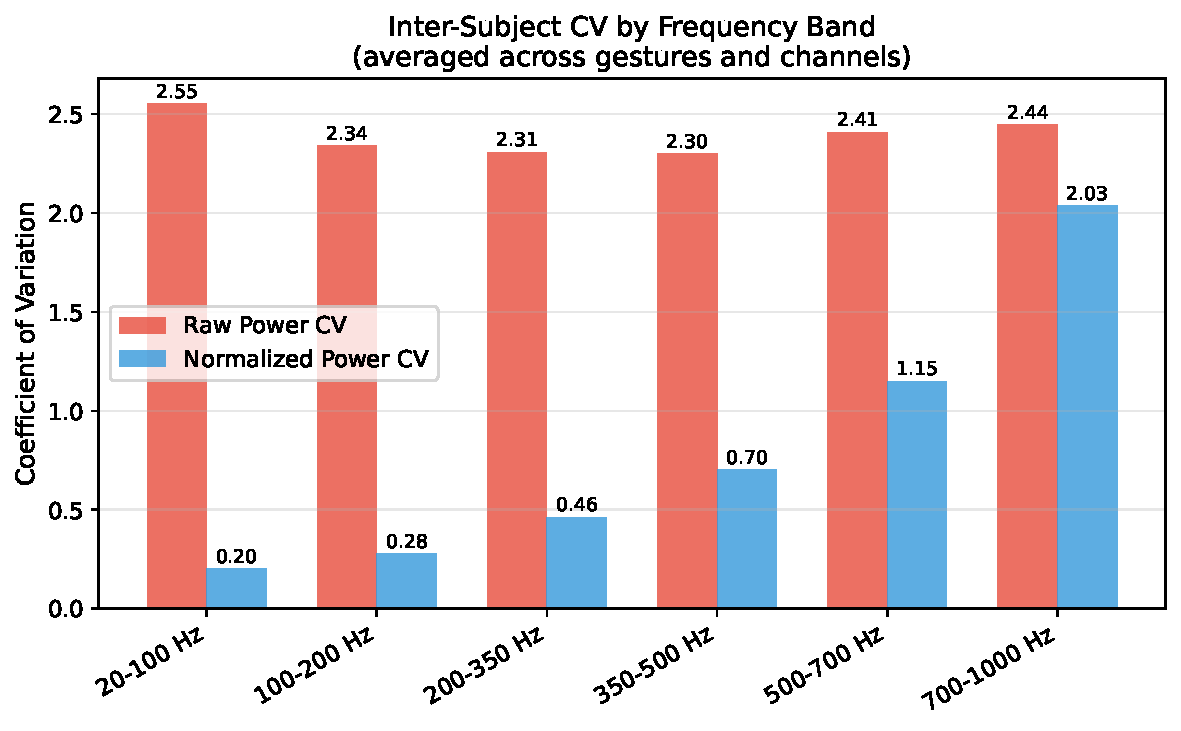
\includegraphics[width=\columnwidth]{fig_h1_cv_by_band.pdf}
\caption{Inter-subject coefficient of variation (CV) by frequency band, averaged over 10~gestures and 12~channels (40~subjects). Red: raw power CV (flat $\sim$2.3--2.6). Blue: normalized CV (power in band / total power), showing a \textbf{tenfold increase} from 20--100\,Hz to 700--1000\,Hz.}
\label{fig:h1_cv}
\end{figure}

\begin{figure}[t]
\centering
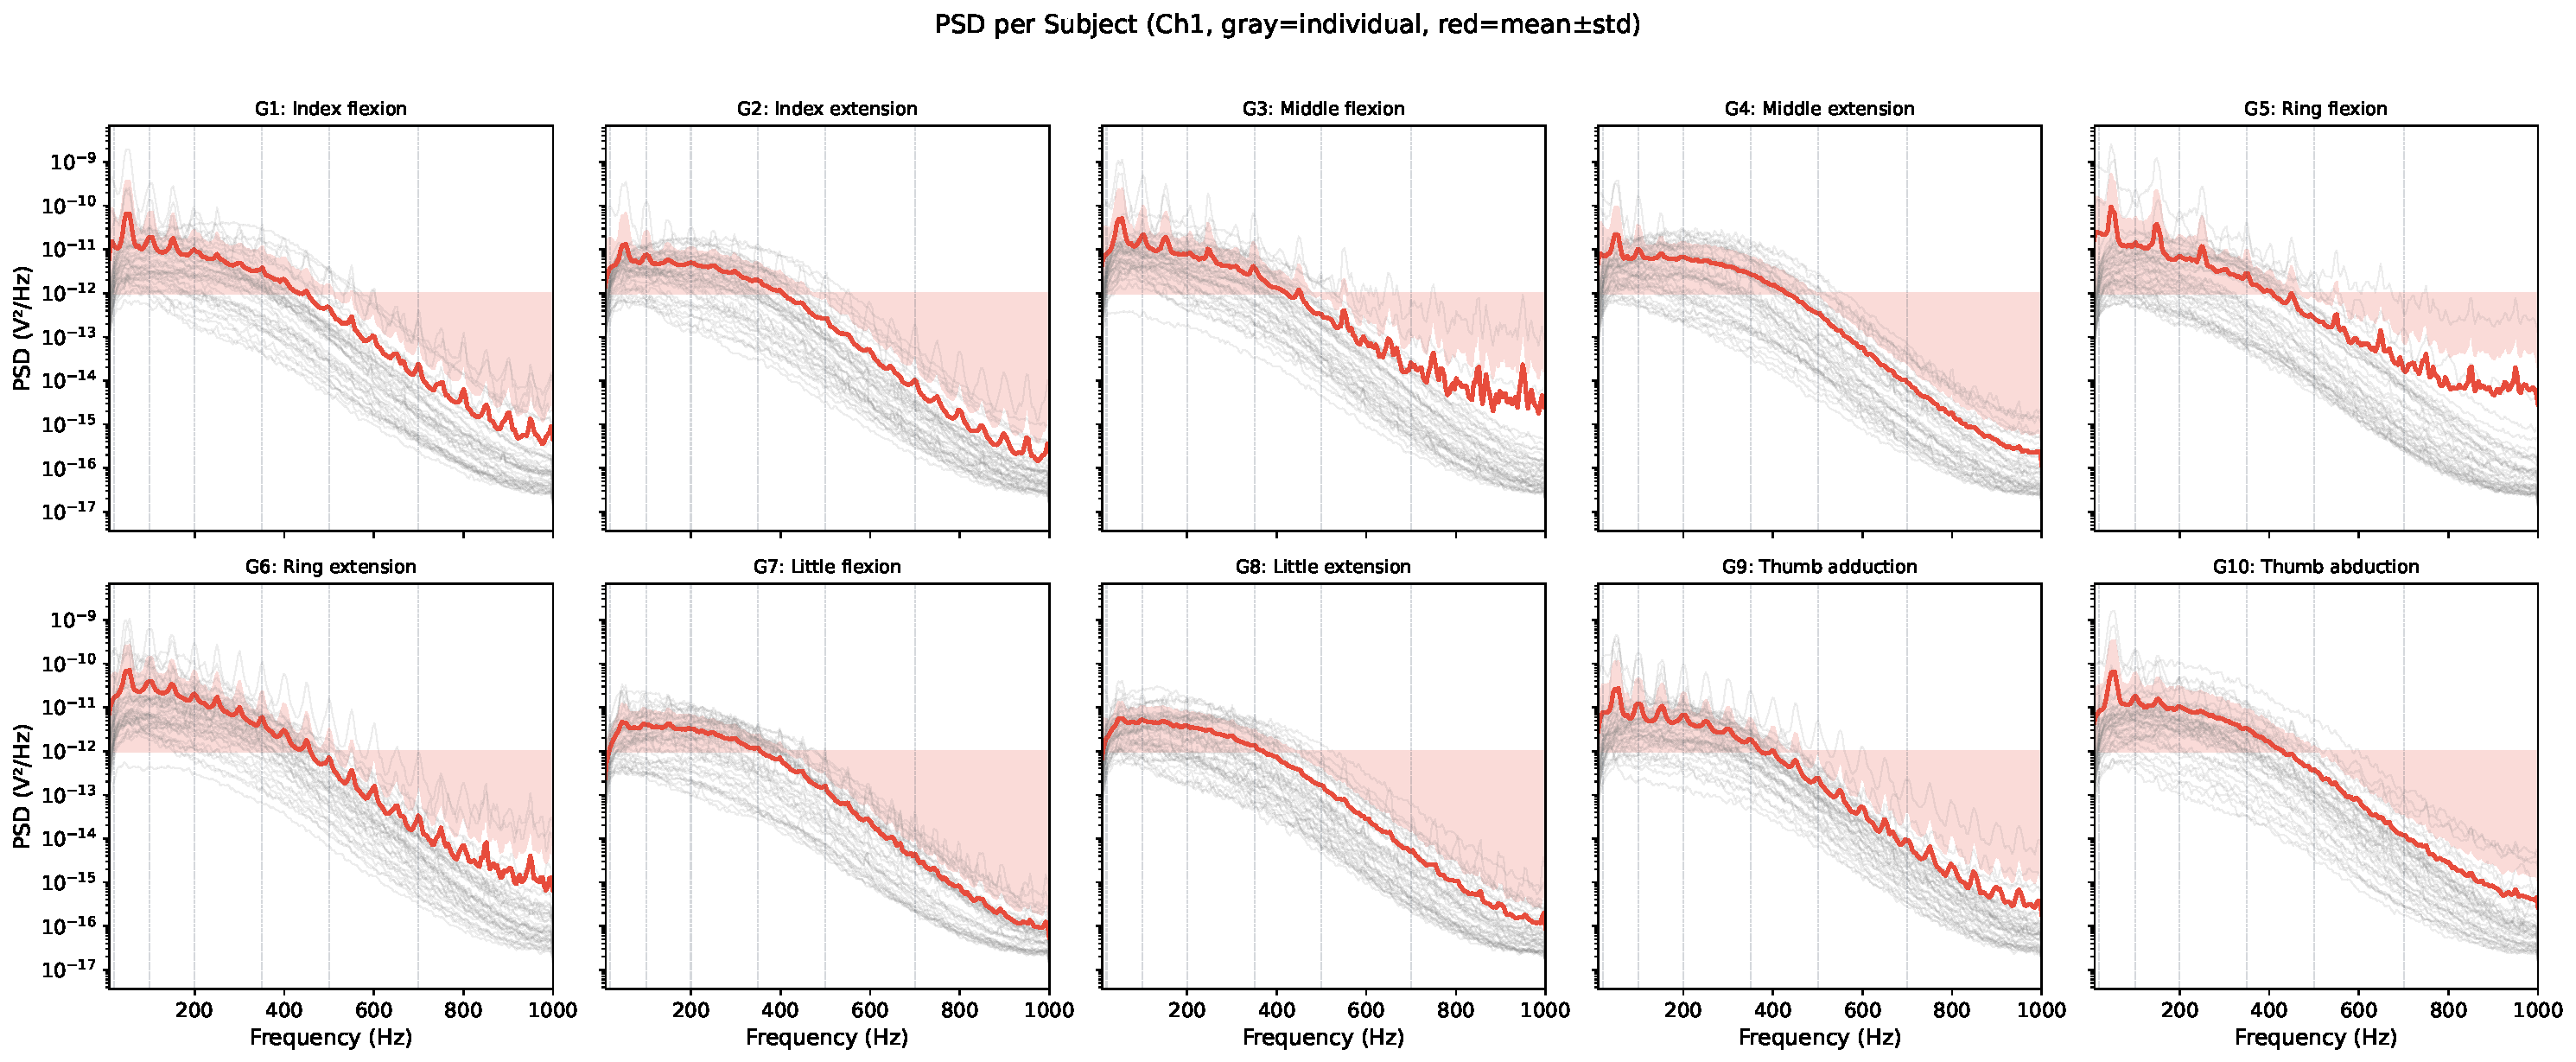
\includegraphics[width=\columnwidth]{fig_h1_psd_overlay.pdf}
\caption{Welch PSD per gesture (Channel~1, 40~subjects). Gray lines: individual subjects; red: mean $\pm$ std. The inter-subject envelope widens non-uniformly across the spectrum, motivating per-band processing.}
\label{fig:h1_psd}
\end{figure}

\textbf{Implication.} A monolithic model that processes all frequencies identically must trade off suppression of high-frequency subject noise against preservation of low-frequency gesture information.
Frequency decomposition allows per-band processing, applying stronger normalization where variability is highest.

% ======================================================================
%  V. METHOD
% ======================================================================
\section{Proposed Method}
\label{sec:method}

\begin{figure}[t]
\centering
\resizebox{\columnwidth}{!}{%
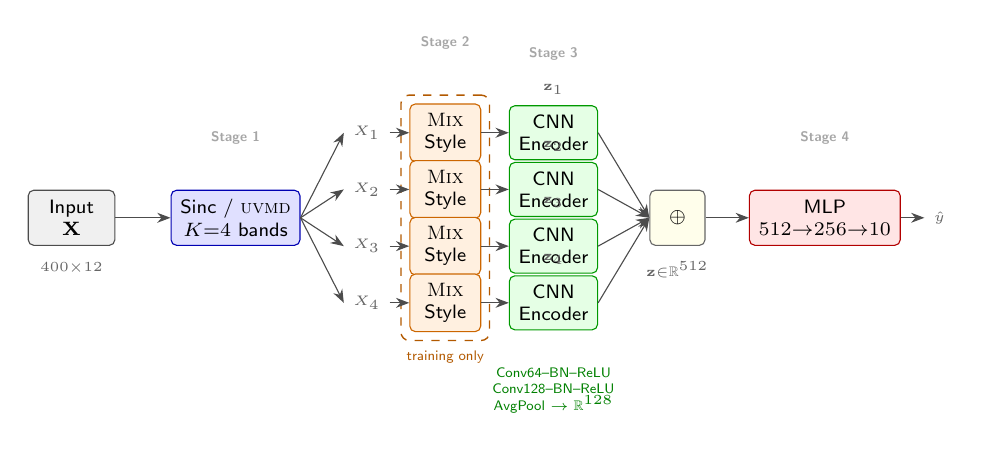
\begin{tikzpicture}[
    >=Stealth,
    node distance=0.45cm and 0.55cm,
    font=\sffamily\scriptsize,
    inputbox/.style={
        rectangle, rounded corners=2pt, draw=black!70, fill=gray!12,
        minimum height=0.7cm, minimum width=1.1cm, align=center,
        line width=0.4pt
    },
    decompbox/.style={
        rectangle, rounded corners=2pt, draw=blue!70!black, fill=blue!12,
        minimum height=0.7cm, minimum width=1.3cm, align=center,
        line width=0.4pt
    },
    mixbox/.style={
        rectangle, rounded corners=2pt, draw=orange!80!black, fill=orange!12,
        minimum height=0.5cm, minimum width=0.9cm, align=center,
        line width=0.4pt
    },
    encbox/.style={
        rectangle, rounded corners=2pt, draw=green!60!black, fill=green!10,
        minimum height=0.5cm, minimum width=1.1cm, align=center,
        line width=0.4pt
    },
    classbox/.style={
        rectangle, rounded corners=2pt, draw=red!70!black, fill=red!10,
        minimum height=0.7cm, minimum width=1.0cm, align=center,
        line width=0.4pt
    },
    concatbox/.style={
        rectangle, rounded corners=2pt, draw=black!60, fill=yellow!8,
        minimum height=0.7cm, minimum width=0.7cm, align=center,
        line width=0.4pt
    },
    arrstyle/.style={->, line width=0.4pt, black!70},
    dimlabel/.style={font=\sffamily\tiny, text=black!60},
]

% ---- Input ----
\node[inputbox] (input) {Input\\$\mathbf{X}$};
\node[dimlabel, below=0.08cm of input] {$400{\times}12$};

% ---- Decomposition ----
\node[decompbox, right=0.7cm of input] (decomp) {Sinc / \textsc{uvmd}\\$K{=}4$ bands};

\draw[arrstyle] (input) -- (decomp);

% ---- Sub-band fan-out: 4 parallel paths ----
\foreach \i/\lab in {1/$X_1$, 2/$X_2$, 3/$X_3$, 4/$X_4$} {
    \pgfmathsetmacro{\yoff}{(2.5 - \i) * 0.72}
    \node[dimlabel, right=0.55cm of decomp, yshift=\yoff cm] (sb\i) {\lab};
}

% Arrows from decomp to sub-band labels
\foreach \i in {1,2,3,4} {
    \draw[arrstyle] (decomp.east) -- (sb\i.west);
}

% ---- MixStyle blocks ----
\foreach \i in {1,2,3,4} {
    \node[mixbox, right=0.25cm of sb\i] (mix\i) {\textsc{Mix}\\Style};
}

\foreach \i in {1,2,3,4} {
    \draw[arrstyle] (sb\i) -- (mix\i);
}

% ---- Dashed "training only" box around MixStyle ----
\begin{scope}[on background layer]
    \node[draw=orange!70!black, dashed, rounded corners=3pt, line width=0.5pt,
          inner sep=3pt, fit=(mix1)(mix4),
          label={[font=\sffamily\tiny, text=orange!70!black]below:training only}] (mixfit) {};
\end{scope}

% ---- Per-band CNN encoders ----
\foreach \i in {1,2,3,4} {
    \node[encbox, right=0.35cm of mix\i] (enc\i) {CNN\\Encoder};
}

\foreach \i in {1,2,3,4} {
    \draw[arrstyle] (mix\i) -- (enc\i);
}

% z_k labels
\foreach \i in {1,2,3,4} {
    \node[dimlabel, above=0.01cm of enc\i, font=\sffamily\tiny] {$\mathbf{z}_\i$};
}

% ---- Concat node ----
\coordinate (encmid) at ($(enc2.east)!0.5!(enc3.east)$);
\node[concatbox, right=0.65cm of encmid] (concat) {$\oplus$};

\foreach \i in {1,2,3,4} {
    \draw[arrstyle] (enc\i.east) -- (concat.west);
}

\node[dimlabel, below=0.08cm of concat] {$\mathbf{z}{\in}\mathbb{R}^{512}$};

% ---- Classifier ----
\node[classbox, right=0.55cm of concat] (cls) {MLP\\$512{\to}256{\to}10$};
\draw[arrstyle] (concat) -- (cls);

% Output
\node[dimlabel, right=0.3cm of cls] (out) {$\hat{y}$};
\draw[arrstyle] (cls) -- (out);

% ---- Encoder detail annotation ----
\node[font=\sffamily\tiny, text=green!50!black, below=0.35cm of enc4,
      align=center, anchor=north]
      {Conv64--BN--ReLU\\Conv128--BN--ReLU\\AvgPool $\to$ $\mathbb{R}^{128}$};

% ---- Stage labels (top) ----
\node[font=\sffamily\tiny\bfseries, text=gray!70, above=0.45cm of decomp] {Stage 1};
\node[font=\sffamily\tiny\bfseries, text=gray!70, above=0.45cm of mixfit] {Stage 2};
\node[font=\sffamily\tiny\bfseries, text=gray!70, above=0.45cm of enc1] {Stage 3};
\node[font=\sffamily\tiny\bfseries, text=gray!70, above=0.45cm of cls] {Stage 4};

\end{tikzpicture}%
}% end resizebox
\iflanguage{russian}{%
\caption{Архитектура предлагаемого частотно-ориентированного конвейера.
Этап~1: декомпозиция входного сигнала на $K{=}4$ частотных поддиапазона (Sinc или \textsc{uvmd}).
Этап~2: побандовый \textsc{MixStyle} (только при обучении; ноль параметров) смешивает статистики между субъектами.
Этап~3: независимое кодирование каждого поддиапазона CNN-энкодером ($\mathbf{z}_k \in \mathbb{R}^{128}$).
Этап~4: классификация конкатенированного представления $\mathbf{z} \in \mathbb{R}^{512}$ MLP-головой.}%
}{%
\caption{Architecture of the proposed frequency-aware sEMG pipeline.
Stage~1 decomposes the raw input into $K{=}4$ frequency sub-bands via either
a fixed Sinc filterbank or learnable \textsc{uvmd}.
Stage~2 applies per-band \textsc{MixStyle} (training only; zero parameters) to
mix channel-wise statistics between subjects.
Stage~3 encodes each sub-band independently through shared-architecture CNN
encoders, producing $\mathbf{z}_k \in \mathbb{R}^{128}$.
The concatenated representation $\mathbf{z} \in \mathbb{R}^{512}$ is classified
by an MLP head (Stage~4).}%
}
\label{fig:architecture}
\end{figure}


Our pipeline (\cref{fig:architecture}) processes a raw sEMG window $\mathbf{X} \in \mathbb{R}^{T \times C}$ ($T$\,=\,400 samples, $C$\,=\,12 channels) in four stages:

\subsection{Stage 1: Frequency Decomposition}
We decompose $\mathbf{X}$ into $K$\,=\,4 sub-band signals $\{\mathbf{X}_k\}_{k=1}^{K}$, each $\in \mathbb{R}^{T \times C}$, using one of two frontends:

\paragraph{Fixed Sinc Filterbank.}
Four bandpass Sinc filters with fixed cutoff frequencies partition the Nyquist band into equal sub-bands.
For filter $k$ with passband $[f_k^{\mathrm{lo}}, f_k^{\mathrm{hi}}]$:
\begin{equation}
h_k[n] = 2f_k^{\mathrm{hi}} \operatorname{sinc}(2f_k^{\mathrm{hi}} n) - 2f_k^{\mathrm{lo}} \operatorname{sinc}(2f_k^{\mathrm{lo}} n)
\label{eq:sinc}
\end{equation}
windowed by a Hamming function, applied via convolution to each channel independently.
The cutoffs are fixed at $[0, 0.125, 0.25, 0.375, 0.5]$ (normalized frequency), corresponding to four equal-width bands.
This frontend adds only 8 parameters (4 pairs of cutoff frequencies).

\paragraph{Unfolded VMD (\uvmd{}).}
We \emph{unroll} $L$\,=\,8 iterations of the alternating direction method of multipliers (ADMM) update for Variational Mode Decomposition~\cite{dragomiretskiy2014variational} into a differentiable neural network block.
The learnable parameters are:
\begin{itemize}
    \item $\boldsymbol{\alpha} \in \mathbb{R}^{L \times K}$: per-iteration, per-mode bandwidth penalty,
    \item $\boldsymbol{\tau} \in \mathbb{R}^{L}$: per-iteration Lagrangian step size,
    \item $\boldsymbol{\omega} \in \mathbb{R}^{K}$: center frequencies (initialized uniformly at $[0.05, 0.18, 0.32, 0.45]$).
\end{itemize}
At each ADMM iteration $l$ and for each mode $k$, the spectral-domain update reads:
\begin{equation}
\hat{u}_k^{(l)}(\xi) = \frac{\hat{r}_k(\xi)}{1 + \alpha_{l,k} (\xi - \omega_k)^2}
\label{eq:uvmd}
\end{equation}
where $\hat{r}_k$ is the residual after removing all other modes.
A spectral overlap penalty $\mathcal{L}_{\mathrm{overlap}} = \sum_{j \neq k} \exp(-10(\omega_j - \omega_k)^2)$ encourages frequency diversity.
This frontend adds 44 parameters ($\boldsymbol{\alpha}$: 32, $\boldsymbol{\tau}$: 8, $\boldsymbol{\omega}$: 4).

\subsection{Stage 2: Per-Band Encoder}
Each sub-band $\mathbf{X}_k$ is independently encoded by a shared-architecture 1D-CNN:
\begin{multline}
\mathbf{z}_k = \operatorname{AvgPool}\!\big(\operatorname{ReLU}\!\big(\operatorname{BN}\!\big( \\
\operatorname{Conv}_{128}\!\big(\operatorname{ReLU}\!\big(\operatorname{BN}\!\big(\operatorname{Conv}_{64}(\mathbf{X}_k)\big)\big)\big)\big)\big)\big)
\end{multline}
where $\operatorname{Conv}_{d}$ denotes $\operatorname{Conv1d}(C, d, \cdot)$ with kernel sizes 5 and 3 respectively, and $\operatorname{AvgPool}$ is global adaptive average pooling.
Each encoder maps $\mathbb{R}^{T \times C} \to \mathbb{R}^{128}$; four encoders yield $\mathbf{z} = [\mathbf{z}_1; \ldots; \mathbf{z}_4] \in \mathbb{R}^{512}$.

\subsection{Stage 3: Per-Band \mixstyle{}}
\label{sec:mixstyle}
During training only, we apply \mixstyle{}~\cite{zhou2021mixstyle} independently to each sub-band \emph{before} encoding.
For sub-band $k$ and sample $i$ in a mini-batch:
\begin{align}
\mu_k^{(i)} &= \mathbb{E}_t[\mathbf{X}_k^{(i)}], \quad
\sigma_k^{(i)} = \sqrt{\operatorname{Var}_t[\mathbf{X}_k^{(i)}] + \epsilon} \label{eq:ms_stats} \\
\tilde{\mathbf{X}}_k^{(i)} &= \frac{\mathbf{X}_k^{(i)} - \mu_k^{(i)}}{\sigma_k^{(i)}} \label{eq:ms_norm} \\
\lambda &\sim \operatorname{Beta}(\alpha, \alpha), \quad j = \operatorname{shuffle}(i) \label{eq:ms_lambda} \\
\tilde{\mu}_k &= \lambda \mu_k^{(i)} + (1-\lambda) \mu_k^{(j)}, \quad
\tilde{\sigma}_k = \lambda \sigma_k^{(i)} + (1-\lambda) \sigma_k^{(j)} \label{eq:ms_mix} \\
\hat{\mathbf{X}}_k^{(i)} &= \tilde{\sigma}_k \cdot \tilde{\mathbf{X}}_k^{(i)} + \tilde{\mu}_k \label{eq:ms_out}
\end{align}
with $\alpha$\,=\,0.1 and application probability $p$\,=\,0.5.
This module has \textbf{zero learnable parameters}: it only manipulates running statistics.
The key distinction from global \mixstyle{} is per-band application, allowing different levels of style perturbation in each frequency range---directly implementing the H1~insight that high-frequency bands require more aggressive normalization.

\paragraph{Adaptive Per-Band \mixstyle{} (H8).}
We extend the fixed module by making $\alpha$ and $p$ \emph{learnable per band}:
\begin{equation}
\alpha_k = \operatorname{softplus}(\theta_k^{\alpha}) + \epsilon, \quad
p_k = \sigma(\theta_k^{p})
\label{eq:adaptive_ms}
\end{equation}
where $\theta_k^{\alpha}, \theta_k^{p}$ are raw parameters initialized to yield $\alpha_k$\,=\,0.1, $p_k$\,=\,0.5.
The output is a soft blend of the original and style-mixed signals:
$\hat{\mathbf{X}}_k = p_k \cdot \tilde{\mathbf{X}}_k^{\mathrm{mixed}} + (1 - p_k) \cdot \mathbf{X}_k$,
making the module fully differentiable via reparameterized Beta sampling.
This adds only $2K$\,=\,8 learnable parameters.

\paragraph{Spectral Content Gate (H9).}
Instead of augmenting style (MixStyle), the \emph{Spectral Content Gate} (SCG) learns to \emph{selectively remove} it.
For each sub-band $k$, a learnable gate $\gamma_k = \sigma(\theta_k^{\gamma}) \in [0, 1]$ blends between the instance-normalized (style-free) and raw (style-preserved) input:
\begin{equation}
\hat{\mathbf{X}}_k = \gamma_k \cdot \frac{\mathbf{X}_k - \mu_k}{\sigma_k} + (1 - \gamma_k) \cdot \mathbf{X}_k
\label{eq:scg}
\end{equation}
When $\gamma_k \to 1$, band $k$ undergoes full Instance Normalization (all style removed); when $\gamma_k \to 0$, the raw signal is preserved.
This adds only $K$\,=\,4 learnable parameters.
The key distinction from MixStyle is that SCG is a \emph{deterministic, inference-time-active} module---it permanently transforms the representation rather than providing training-time augmentation.

\subsection{Stage 4: Classifier}
A two-layer MLP maps $\mathbf{z} \in \mathbb{R}^{512}$ to class logits:
$512 \to 256$ (ReLU, dropout $p$\,=\,0.3) $\to$ 10 (softmax).

\paragraph{Training.}
The total loss is:
\begin{equation}
\mathcal{L} = \mathcal{L}_{\mathrm{CE}} + \lambda_{\mathrm{ov}} \cdot \mathcal{L}_{\mathrm{overlap}}
\end{equation}
with $\lambda_{\mathrm{ov}}$\,=\,0.01 (for \uvmd{} only; zero for Sinc).
We use Adam ($\mathrm{lr}$\,=\,$10^{-3}$), ReduceLROnPlateau (factor 0.5, patience 5), and early stopping (patience 15) for up to 80~epochs.

\paragraph{Model size.}
\Cref{tab:params} summarizes parameter counts.
The decomposition frontend adds negligible overhead (8--44 parameters); the dominant cost is the four per-band encoders (116\,000).
\mixstyle{} adds zero parameters.

\begin{table}[t]
\centering
\caption{Parameter count by model variant.}
\label{tab:params}
\resizebox{\columnwidth}{!}{%
\begin{tabular}{lrrl}
\toprule
Variant & Total & Frontend & Note \\
\midrule
A: Raw CNN ($K$=1) & 64\,586 & 0 & Single encoder \\
B: Sinc FB ($K$=4) & 249\,874 & 8 & 4 encoders \\
C: Sinc + \mixstyle{} & 249\,874 & 8 & +0 for \mixstyle{} \\
D: Sinc + MS + CS heads & 172\,130 & 8 & Content/style split \\
E/F: \uvmd{} ($K$=4) & 249\,910 & 44 & Learnable decomp. \\
G: Sinc + Adaptive MS & 249\,882 & 16 & +8 for $\alpha_k, p_k$ \\
H: \uvmd{} + Adaptive MS & 249\,918 & 52 & +8 for $\alpha_k, p_k$ \\
SCG-A: Sinc + SCG & 136\,974 & 12 & +4 for $\gamma_k$ \\
SCG-B: \uvmd{} + SCG + Adv & 172\,365 & 48 & +4 $\gamma_k$, +35K adv. \\
\bottomrule
\end{tabular}%
}
\end{table}

% ======================================================================
%  VI. EXPERIMENTS AND RESULTS
% ======================================================================
\section{Experiments and Results}
\label{sec:results}

\subsection{Hypothesis Chain Overview}
\Cref{tab:hypotheses} summarizes the nine hypotheses, their status, and key results.
Each hypothesis builds on the conclusions of the previous one, forming a coherent investigative chain.
$p$-values are corrected via the Holm--Bonferroni procedure within pre-defined hypothesis families (see \cref{sec:stats}).

\begin{table*}[t]
\centering
\caption{Hypothesis chain summary. NinaPro DB2 E1, 20 subjects, strict LOSO. $p_{\mathrm{Holm}}$: Holm-corrected within hypothesis family. Status: \textbf{C}~=~confirmatory ($p_{\mathrm{Holm}}$\,$<$\,0.05), \textbf{E}~=~exploratory ($p_{\mathrm{uncorr.}}$\,$<$\,0.05 only), \textbf{R}~=~rejected, \textbf{D}~=~descriptive. Family labels: A=decomposition, B=soft~style, C=hard~norm, D=disentanglement, E=SCG-Net. $\dagger$H2--H5: batch=64; H6--H9: batch=512 (see \cref{sec:batchsize}).}
\label{tab:hypotheses}
\begin{tabular}{clp{4.8cm}ccccc}
\toprule
\# & Hypothesis & Key Question & Family & Status & Best $\Delta$F1 & $p_{\mathrm{uncorr.}}$ & $p_{\mathrm{Holm}}$ \\
\midrule
H1 & Spectral variability & Is inter-subject variability frequency-dependent? & --- & \textbf{D} & --- & --- & --- \\
H2$^\dagger$ & Decomposition & Does freq.\ decomposition beat raw signal? & A & \textbf{C} & +2.3\pp{} & 0.007 & $<$0.02 \\
H3$^\dagger$ & Style normalization & Does per-band \mixstyle{} help? & B & \textbf{E} & +1.7\pp{} & 0.04 & 0.08 \\
   &                     & Does Instance Norm help? & C & \textbf{R (C)} & $-$7.0\pp{} & $<$0.001 & $<$0.002 \\
H4$^\dagger$ & Disentanglement & Does explicit content/style separation help? & D & \textbf{R (C)} & $-$2.6\pp{} & $<$0.001 & $<$0.004 \\
H5$^\dagger$ & Architecture & Do $K$\,$>$\,4, SE-attention, or DRO help? & --- & \textbf{R} & $-$0.3\pp{} & $>$0.13 & --- \\
H6 & Unified ablation & Decomposition contribution (A$\to$B) & A & \textbf{C} & +3.7\pp{} & $<$0.001 & $<$0.003 \\
   &                   & \mixstyle{} contribution (B$\to$C) & B & \textbf{E} & +1.1\pp{} & 0.07 & 0.07 \\
H7 & \uvmd{} + \mixstyle{} & Is \mixstyle{} frontend-agnostic? & B & \textbf{C} & +1.8\pp{} & 0.003 & $<$0.01 \\
H8 & Adaptive \mixstyle{} & Does the network learn the H1 gradient? & --- & \textbf{D$^{\ddagger}$} & +0.97\pp{} & 0.064 & --- \\
H9 & SCG-Net & Does per-band gate outperform uniform IN? & E & \textbf{C} & +6.86\pp{} & $<$0.001 & $<$0.001 \\
\bottomrule
\multicolumn{8}{l}{\footnotesize $\ddagger$H8 is descriptive: primary evidence is the learned parameter gradient (Spearman $\rho$\,=\,0.78, $p$\,$<$\,$10^{-16}$), not $\Delta$F1.}
\end{tabular}
\end{table*}

\subsection{H2: Frequency Decomposition vs.\ Raw Signal}

\Cref{tab:h2} shows that $K$\,=\,4 decomposition consistently outperforms raw-signal processing.
Both Sinc filterbank and \uvmd{} yield +2.1--2.3\pp{} F1 improvement with medium effect sizes ($d$\,$\approx$\,0.67--0.68).
Within Family~A (decomposition, $k$\,=\,3), both comparisons reach significance after Holm correction ($p_{\mathrm{Holm}}$\,$<$\,0.02), and the controlled H6~ablation (\cref{sec:h6}) independently confirms the effect ($p_{\mathrm{Holm}}$\,$<$\,0.003).
Sinc and \uvmd{} are statistically indistinguishable ($\Delta$\,=\,+0.24\pp{}, $p$\,=\,0.50), motivating the use of the simpler Sinc frontend in subsequent experiments.

\emph{Note on experimental series.}
H2--H5 were conducted with batch\_size\,=\,64; H6--H7 with batch\_size\,=\,512.
This difference affects absolute F1 values (see \cref{sec:batchsize}) and means that results from different series should not be compared directly across tables.

\begin{table}[t]
\centering
\caption{H2: Decomposition comparison (20 subjects, LOSO).}
\label{tab:h2}
\begin{tabular}{lccc}
\toprule
Frontend & F1 (\%) & $\Delta$ vs.\ raw & $d$ \\
\midrule
None (raw) & 34.90 $\pm$ 8.16 & --- & --- \\
Sinc FB ($K$=4) & 37.00 $\pm$ 7.56 & +2.10 & 0.67 \\
\uvmd{} ($K$=4) & 37.24 $\pm$ 7.75 & +2.34 & 0.68 \\
\bottomrule
\end{tabular}
\end{table}

\subsection{H3: Per-Band Style Normalization}

\Cref{tab:h3} reveals an asymmetry between soft and hard normalization.
Per-band \mixstyle{} yields +1.67\pp{} with medium effect size ($d$\,=\,0.54), but does not reach significance after Holm correction within Family~B ($p_{\mathrm{Holm}}$\,=\,0.08; $p_{\mathrm{uncorr.}}$\,=\,0.04); we treat this as exploratory evidence.
In contrast, hard Instance Normalization (Family~C) causes large, statistically confirmed degradation: global IN loses $-$7.0\pp{} ($p_{\mathrm{Holm}}$\,$<$\,0.002, $d$\,=\,$-$1.13); per-band IN is worse at $-$8.5\pp{} ($p_{\mathrm{Holm}}$\,$<$\,0.002, $d$\,=\,$-$1.36).

The adaptive IN variant, which learns a per-band normalization strength $\gamma_k$, provides a useful diagnostic: it converges to $\gamma_1$\,=\,0.027 (low-frequency) versus $\gamma_4$\,=\,0.38 (high-frequency)---a 14:1 ratio consistent with the H1~observation that high-frequency bands carry more subject-specific variation.

\begin{table}[t]
\centering
\caption{H3: Style normalization comparison (20 subjects, LOSO). Baseline: Sinc FB ($K$=4), no normalization.}
\label{tab:h3}
\begin{tabular}{lccc}
\toprule
Normalization & F1 (\%) & $\Delta$ & $d$ \\
\midrule
None (baseline) & 36.28 $\pm$ 7.81 & --- & --- \\
Per-band \mixstyle{} & \textbf{37.95 $\pm$ 7.22} & +1.67 & 0.54 \\
Adaptive IN ($\gamma_k$) & 36.90 $\pm$ 6.98 & +0.62 & 0.24 \\
Global IN & 29.29 $\pm$ 5.30 & $-$6.99 & $-$1.13 \\
Per-band IN & 27.75 $\pm$ 4.29 & $-$8.53 & $-$1.36 \\
\bottomrule
\end{tabular}
\end{table}

\subsection{H4: Content--Style Disentanglement}

Starting from the H3 configuration with content/style projection heads (Sinc FB + \mixstyle{} + CS heads, F1\,=\,39.19\%; note this differs from the \mixstyle{}-only result of 37.95\% in \cref{tab:h3} because H4 uses a modified architecture with separate content and style encoders), we test whether explicit disentanglement losses can improve generalization (\cref{tab:h4}).
All auxiliary losses \emph{degrade} performance:

\begin{table}[t]
\centering
\caption{H4: Effect of auxiliary disentanglement losses (20 subjects). Baseline: Sinc FB + \mixstyle{} (no auxiliary losses).}
\label{tab:h4}
\begin{tabular}{lcccc}
\toprule
Auxiliary Loss & F1 (\%) & $\Delta$ & $d$ & $p_{\mathrm{Holm}}$ \\
\midrule
None (baseline) & \textbf{39.19 $\pm$ 6.34} & --- & --- & --- \\
+ Contrastive & 38.99 $\pm$ 5.95 & $-$0.19 & $-$0.14 & 1.00 \\
+ Adversarial (GRL) & 36.60 $\pm$ 5.99 & $-$2.58 & $-$2.16 & $<$0.004 \\
+ MI minimization & 35.29 $\pm$ 7.28 & $-$3.89 & $-$0.97 & $<$0.01 \\
+ All combined & 34.89 $\pm$ 7.18 & $-$4.30 & $-$1.04 & $<$0.01 \\
\bottomrule
\end{tabular}
\end{table}

The adversarial loss (gradient reversal layer) worsens every subject (0/20 improved, $d$\,=\,$-$2.16, $p_{\mathrm{Holm}}$\,$<$\,0.004).
This suggests that, in our setting, gesture content and subject style share sufficient information that forcing their separation degrades the representation.
\emph{Implicit} style robustness via \mixstyle{} appears preferable to \emph{explicit} content--style separation, at least under this architecture and training regime.

\subsection{H5: Architecture Optimization}

We test whether increasing model capacity ($K$\,=\,6, $K$\,=\,8), adding Squeeze-and-Excitation attention, or GroupDRO loss can improve upon the $K$\,=\,4 baseline.
Friedman test across six variants yields $\chi^2$\,=\,2.94, $p$\,=\,0.71---no significant differences.
The best variant ($K$\,=\,4, no additions, F1\,=\,39.75\%) remains the simplest.
Within the range of architectures tested, additional complexity does not improve performance; however, this does not rule out gains from fundamentally different architectures or training strategies.

\subsection{H6: Unified Ablation (Component Attribution)}
\label{sec:h6}

To isolate individual component contributions, we fix a single backbone architecture and vary one component per step (\cref{tab:h6}).
Note that H6--H7 use batch\_size\,=\,512 (vs.\ 64 in H2--H5), which affects absolute F1 values and limits direct cross-table comparison (see \cref{sec:batchsize}).

\begin{table}[t]
\centering
\caption{H6: Unified ablation (20 subjects, batch=512, LOSO). Each step adds exactly one component. Statistical tests: Wilcoxon with Holm correction within hypothesis families (A, B).}
\label{tab:h6}
\resizebox{\columnwidth}{!}{%
\begin{tabular}{llcccccc}
\toprule
& Components & F1 (\%) & IQR & $\Delta_{\mathrm{step}}$ & $d$ & $p_{\mathrm{Holm}}$ & $\uparrow/\downarrow$ \\
\midrule
A & Raw CNN & 32.40 $\pm$ 5.91 & 8.9 & --- & --- & --- & --- \\
B & + Sinc FB & 36.08 $\pm$ 7.29 & 10.4 & +3.68 & 1.25 & $<$0.003 & 18/2 \\
C & + \mixstyle{} & \textbf{37.19 $\pm$ 6.21} & 8.5 & +1.11 & 0.42 & 0.07$^*$ & 18/2 \\
D & + CS heads & 36.37 $\pm$ 6.07 & 8.8 & $-$0.82 & $-$0.62 & 0.34 & 5/15 \\
\bottomrule
\multicolumn{8}{l}{\footnotesize $^*$Exploratory: does not reach significance within Family~B.}
\end{tabular}%
}
\end{table}

\textbf{Key findings:}
\begin{itemize}
    \item \textbf{Decomposition} (A$\to$B): +3.68\pp{}, $d$\,=\,1.25 (large), $p_{\mathrm{Holm}}$\,$<$\,0.003 (Family~A). Confirmatory.
    \item \textbf{\mixstyle{}} (B$\to$C): +1.11\pp{}, $d$\,=\,0.42 (small--medium), $p_{\mathrm{uncorr.}}$\,=\,0.07. Consistent direction (18/20 subjects improve) but does not reach significance. Exploratory.
    \item \textbf{Content/Style heads} (C$\to$D): $-$0.82\pp{}, harmful (15/20 worsen).
\end{itemize}

The best-performing variant within this ablation is \textbf{Variant~C} (Sinc filterbank + per-band \mixstyle{}), though the marginal contribution of \mixstyle{} over decomposition alone is not individually confirmed after correction.

\subsection{H7: Per-Band \mixstyle{} on Learnable Decomposition}

Does \mixstyle{} help only with fixed decomposition, or does it generalize to learnable frontends?
We test on \uvmd{} (\cref{tab:h7}).

\begin{table}[t]
\centering
\caption{H7: \uvmd{} + \mixstyle{} (20 subjects, batch=512, LOSO; Variant~F replicated at batch=64 with $p$\,=\,0.67). E$\to$F: $p_{\mathrm{Holm}}$\,$<$\,0.01 (Family~B, confirmatory).}
\label{tab:h7}
\resizebox{\columnwidth}{!}{%
\begin{tabular}{llcccc}
\toprule
& Frontend + Style & F1 (\%) & $\Delta$ & $d$ & $p_{\mathrm{uncorr.}}$ \\
\midrule
E & \uvmd{} & 35.79 $\pm$ 6.67 & --- & --- & --- \\
F & \uvmd{} + \mixstyle{} & \textbf{37.58 $\pm$ 6.39} & +1.79 & 0.84 & 0.003 \\
\midrule
& \multicolumn{5}{l}{\textit{Cross-frontend comparison:}} \\
B & Sinc FB & 36.08 $\pm$ 7.29 & \multirow{2}{*}{---} & \multirow{2}{*}{$-$0.16} & \multirow{2}{*}{0.78} \\
E & \uvmd{} & 35.79 $\pm$ 6.67 & & & \\
C & Sinc + MS & 37.19 $\pm$ 6.21 & \multirow{2}{*}{+0.39} & \multirow{2}{*}{0.25} & \multirow{2}{*}{0.43} \\
F & \uvmd{} + MS & 37.58 $\pm$ 6.39 & & & \\
\bottomrule
\end{tabular}%
}
\end{table}

\mixstyle{} adds +1.79\pp{} on \uvmd{} ($d$\,=\,0.84, large effect size).
Within Family~B ($k$\,=\,3), H7 is the smallest $p$-value (0.003) and passes the Holm step ($p_{\mathrm{Holm}}$\,$<$\,0.01), making this a \textbf{confirmatory} result: per-band \mixstyle{} significantly improves the learnable frontend.
However, the sequential Holm procedure stops at the next comparison (H3, $p_{\mathrm{uncorr.}}$\,=\,0.04\,$>$\,$\alpha/2$\,=\,0.025), so the effect on the fixed frontend remains exploratory.
The effect is numerically larger on learnable decomposition (+1.79\pp{}) than on fixed (+1.11\pp{}), possibly because \uvmd{}'s adaptive frequency placement creates sub-bands where style statistics are more informative, though this difference is not tested.

Sinc and \uvmd{} frontends remain statistically indistinguishable ($p$\,=\,0.78 without \mixstyle{}, $p$\,=\,0.43 with), with UVMD better for 10/20 subjects and Sinc for 10/20.
As a batch-size robustness check, Variant~F was replicated at batch\_size\,=\,64: 37.69\%\,$\pm$\,6.85 (paired Wilcoxon $p$\,=\,0.67 vs.\ the bs=512 result), confirming that the finding is not an artifact of batch size (see \cref{sec:batchsize}).

\paragraph{Learned \uvmd{} frequencies.}
\Cref{fig:omega_psd} shows the learned center frequencies overlaid on the EMG power spectrum.
Starting from uniform initialization at [100, 367, 633, 900]\,Hz, \uvmd{} converges to [87$\pm$4, 385$\pm$4, 671$\pm$4, 889$\pm$9]\,Hz across all 20~subjects (std\,$<$\,10\,Hz), indicating a \emph{universal}, subject-independent frequency decomposition.
Mode~1 shifts toward the motor-unit firing band; Mode~2 centers on peak EMG power.

\begin{figure}[t]
\centering
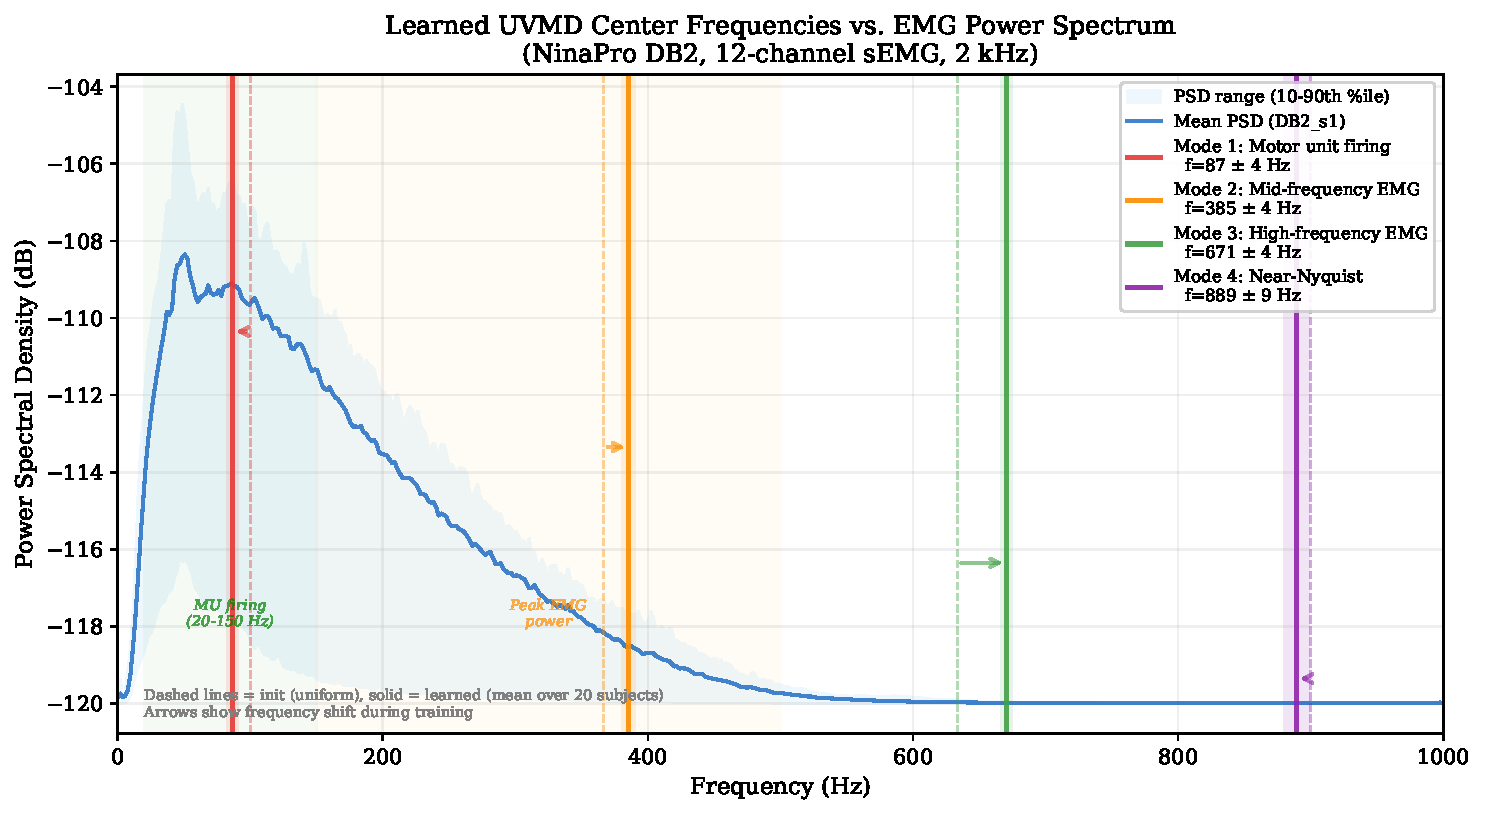
\includegraphics[width=\columnwidth]{fig_uvmd_omega_psd.pdf}
\caption{Learned \uvmd{} center frequencies (solid lines, mean over 20 subjects) overlaid on EMG PSD (representative subject). Dashed lines: initial (uniform) frequencies. Arrows show adaptation direction.}
\label{fig:omega_psd}
\end{figure}

\subsection{H8: Adaptive Per-Band \mixstyle{}}
\label{sec:h8}

Does the network \emph{learn} the frequency-dependent style augmentation implied by H1, or is the fixed $\alpha$\,=\,0.1, $p$\,=\,0.5 already optimal?
We replace the fixed per-band \mixstyle{} with the adaptive variant (\cref{eq:adaptive_ms}) on both Sinc (variant~G) and \uvmd{} (variant~H) frontends.
The MixStyle parameters receive $10\times$ the base learning rate to ensure convergence within 80~epochs.
As an ablation, we also test \emph{reversed-gradient} variants (I, J) that use the learned $\alpha_k, p_k$ values in \emph{reversed band order} (band~4's values assigned to band~1 and vice versa), to verify that the specific band assignment is causally important.

\begin{table}[t]
\centering
\caption{H8: Adaptive Per-Band \mixstyle{} (20 subjects, batch=512, LOSO). G/H: learnable $\alpha_k, p_k$; I/J: reversed-gradient ablation (learned values in wrong band order).}
\label{tab:h8}
\resizebox{\columnwidth}{!}{%
\begin{tabular}{llccc}
\toprule
& Frontend + Style & F1 (\%) & Acc (\%) & $\Delta$F1 vs.\ rev. \\
\midrule
G & Sinc + \textbf{Adaptive MS} & \textbf{35.56 $\pm$ 7.05} & \textbf{37.23 $\pm$ 6.59} & +0.24 \\
I & Sinc + Reversed MS & 35.32 $\pm$ 7.32 & 36.97 $\pm$ 6.62 & --- \\
\midrule
H & \uvmd{} + \textbf{Adaptive MS} & \textbf{34.42 $\pm$ 6.91} & \textbf{36.79 $\pm$ 6.29} & +0.97 \\
J & \uvmd{} + Reversed MS & 33.46 $\pm$ 6.40 & 35.53 $\pm$ 6.02 & --- \\
\bottomrule
\end{tabular}%
}
\end{table}

\Cref{tab:h8} shows that the correct band ordering outperforms the reversed ordering on both frontends.
The effect is stronger on \uvmd{} (+0.97\pp{}, Wilcoxon $p$\,=\,0.064, 15/20~subject wins) than on Sinc (+0.24\pp{}, $p$\,=\,0.67).
The primary finding, however, is not the F1~difference but the \emph{learned parameter gradient} (\cref{tab:h8_params}).

\begin{table}[t]
\centering
\caption{Learned Adaptive \mixstyle{} parameters (mean $\pm$ std across 20 LOSO folds). Init: $\alpha_k$\,=\,0.1, $p_k$\,=\,0.5 for all bands.}
\label{tab:h8_params}
\resizebox{\columnwidth}{!}{%
\begin{tabular}{ccccc}
\toprule
Band & \multicolumn{2}{c}{G (Sinc)} & \multicolumn{2}{c}{H (\uvmd{})} \\
\cmidrule(lr){2-3} \cmidrule(lr){4-5}
$k$ & $\alpha_k$ & $p_k$ & $\alpha_k$ & $p_k$ \\
\midrule
1 (low)  & 1.62 $\pm$ 0.10 & $<$0.001 & 1.30 $\pm$ 0.30 & 0.018 $\pm$ 0.027 \\
2        & 0.89 $\pm$ 0.11 & $<$0.001 & 1.08 $\pm$ 0.24 & 0.014 $\pm$ 0.022 \\
3        & \textbf{7.80 $\pm$ 1.24} & 0.010 $\pm$ 0.002 & \textbf{3.04 $\pm$ 1.45} & 0.036 $\pm$ 0.029 \\
4 (high) & \textbf{16.28 $\pm$ 2.43} & \textbf{0.040 $\pm$ 0.006} & \textbf{2.62 $\pm$ 1.36} & \textbf{0.046 $\pm$ 0.051} \\
\midrule
\multicolumn{1}{l}{Ratio $k$\,=\,4/$k$\,=\,1} & \textbf{10.0$\times$} & $>$100$\times$ & 2.0$\times$ & 2.5$\times$ \\
\multicolumn{1}{l}{Spearman $\rho$} & \multicolumn{2}{c}{0.775 ($p$\,$<$\,$10^{-16}$)} & \multicolumn{2}{c}{0.347 ($p$\,=\,0.002)} \\
\bottomrule
\end{tabular}%
}
\end{table}

Both frontends exhibit a \emph{monotonic gradient} in the learned parameters:
\begin{itemize}
    \item \textbf{$\alpha_k$ increases with frequency}: from 1.62 (band~1) to 16.28 (band~4) on Sinc (\textbf{10$\times$}), and from 1.30 to 2.62 on \uvmd{} (2$\times$). Higher $\alpha$ produces a more concentrated Beta distribution, meaning style mixing becomes less random in high-frequency bands.
    \item \textbf{$p_k$ increases with frequency}: from $<$0.001 to 0.040 on Sinc, from 0.018 to 0.046 on \uvmd{}. The network effectively disables style mixing in low-frequency bands and enables it selectively in high-frequency bands.
\end{itemize}
Spearman rank correlation between band index and $\alpha_k$ is $\rho$\,=\,0.775 ($p$\,$<$\,$10^{-16}$) on Sinc and $\rho$\,=\,0.347 ($p$\,=\,0.002) on \uvmd{}.
This pattern is consistent across all 20~LOSO folds and both frontends.

\paragraph{Interpretive caveats.}
The H8 evidence is \emph{descriptive}, not confirmatory: the Spearman correlation quantifies a pattern in learned parameters, not a controlled manipulation.
The parameters are optimized jointly with all other weights; we cannot rule out that the monotonic gradient is an indirect consequence of other architectural or data properties rather than a direct encoding of the H1~variability structure.
The reversed-gradient ablation provides a partial causal control (correct ordering outperforms reversed on UVMD, $p_{\mathrm{uncorr.}}$\,=\,0.064, 15/20 wins), but the effect is small (+0.97\pp{}) and does not reach significance.
We interpret H8 as \emph{suggestive} evidence that complements, but does not independently confirm, the H1~observation.

\subsection{H9: Spectral Content Gate Network (SCG-Net)}
\label{sec:h9}

Can the H1 insight be encoded directly as an \emph{architectural prior} rather than a training-time augmentation?
SCG-Net replaces MixStyle with the Spectral Content Gate (\cref{eq:scg}): a per-band learnable gate $\gamma_k$ that blends between instance-normalized (style-free) and raw input, adding only $K$\,=\,4 parameters.

\begin{table}[t]
\centering
\caption{H9: SCG-Net results (20 subjects, batch=512, LOSO). Variant~C is the main architecture; A adds a subject adversary; D uses fixed $\gamma_k$\,=\,1 (uniform Instance Norm, ablation).}
\label{tab:h9}
\resizebox{\columnwidth}{!}{%
\begin{tabular}{llccc}
\toprule
& Configuration & F1 (\%) & Acc (\%) & $\Delta$F1 vs.\ D \\
\midrule
SCG-C & Sinc + \textbf{SCG} (learned $\gamma_k$) & \textbf{35.65 $\pm$ 6.60} & \textbf{37.39 $\pm$ 6.07} & +6.86 \\
SCG-A & Sinc + SCG + Adversary & 34.75 $\pm$ 5.92 & 36.17 $\pm$ 5.82 & +5.97 \\
SCG-B & \uvmd{} + SCG + Adversary & 34.56 $\pm$ 5.97 & 36.01 $\pm$ 5.65 & +5.77 \\
SCG-D & Sinc + full IN ($\gamma_k$\,=\,1 fixed) & 28.79 $\pm$ 4.09 & 29.32 $\pm$ 3.94 & --- \\
\bottomrule
\end{tabular}%
}
\end{table}

\begin{table}[t]
\centering
\caption{Learned SCG gate values $\gamma_k$ (mean $\pm$ std across 20 LOSO folds). Init: $\gamma_k$\,=\,0.5 for all bands.}
\label{tab:scg_gates}
\begin{tabular}{ccc}
\toprule
Band $k$ & SCG-C (Sinc) & SCG-A (Sinc + Adv) \\
\midrule
1 (low)  & $<$0.001 & $<$0.001 \\
2        & $<$0.001 & $<$0.001 \\
3        & $<$0.001 & 0.001 $\pm$ 0.001 \\
4 (high) & \textbf{0.998 $\pm$ 0.002} & \textbf{0.910 $\pm$ 0.184} \\
\midrule
Spearman $\rho$ & 0.433 ($p$\,$<$\,$10^{-4}$) & 0.774 ($p$\,$<$\,$10^{-16}$) \\
\bottomrule
\end{tabular}
\end{table}

\Cref{tab:h9} shows that SCG-Net (variant~C) achieves 35.65\% F1, significantly outperforming uniform Instance Normalization (variant~D, 28.79\%) by +6.86\pp{} ($p_{\mathrm{Holm}}$\,$<$\,0.001, Family~E, 18/20~subject wins).
The learned gate values (\cref{tab:scg_gates}) reveal a near-binary partition: $\gamma_{1\text{--}3}$\,$<$\,0.001 (preserve all style in low-frequency bands) and $\gamma_4$\,=\,0.998 (remove style in the highest band).
This pattern is consistent with the H1~observation, though it is learned within the same architectural framework rather than constituting a fully independent validation.

The subject adversary (variant~A) slightly reduces performance compared to SCG without adversary (C), consistent with the H4 finding that adversarial disentanglement can harm sEMG classification.
Wilcoxon test confirms this difference is significant ($p$\,=\,0.048, 12/20~wins for~C over~A).

\subsection{Comparison with Published Baselines}

\Cref{tab:benchmark} compares our results with the published LOSO baselines from Golovan and Zvereva~\cite{golovan2025benchmark}.
Our best variant (\uvmd{}+\mixstyle{}) yields 37.7\% F1 (37.69\% at bs=64, 37.58\% at bs=512), compared with the previous best (CNN/LSTM BiGRU, 33.5\%).
Note that the comparison is between different architectures and training regimes; no paired statistical test is possible since the baselines were trained separately.

\begin{table}[t]
\centering
\caption{Comparison with published baselines (LOSO, 20 subjects, NinaPro DB2 E1). Published results from~\cite{golovan2025benchmark}. $^\dagger$Replication run at batch=64.}
\label{tab:benchmark}
\begin{tabular}{llcc}
\toprule
Method & Features & F1 (\%) \\
\midrule
CNN/LSTM BiGRU~\cite{golovan2025benchmark} & Raw EMG & 33.5 $\pm$ 8.0 \\
Simple CNN~\cite{golovan2025benchmark} & Raw EMG & 33.3 $\pm$ 9.1 \\
SVM-RBF~\cite{golovan2025benchmark} & TD Feat. & 32.6 $\pm$ 7.7 \\
SVM-Linear~\cite{golovan2025benchmark} & TD Feat. & 32.5 $\pm$ 9.4 \\
\midrule
Ours: Sinc + \mixstyle{} (C) & Raw EMG & 37.19 $\pm$ 6.21 \\
\textbf{Ours: \uvmd{} + \mixstyle{} (F)} & \textbf{Raw EMG} & \textbf{37.69 $\pm$ 6.85}$^\dagger$ \\
\bottomrule
\end{tabular}
\end{table}

\subsection{Who Benefits from \mixstyle{}?}

\Cref{fig:mixstyle_corr} shows that \mixstyle{}'s benefit correlates negatively with baseline F1 for the Sinc frontend ($r$\,=\,$-$0.56, $p$\,=\,0.01): weaker subjects gain more, while strong subjects see diminishing returns.
This suggests that \mixstyle{} acts as a regularizer, primarily helping subjects whose signals deviate most from the training distribution.

\begin{figure}[t]
\centering
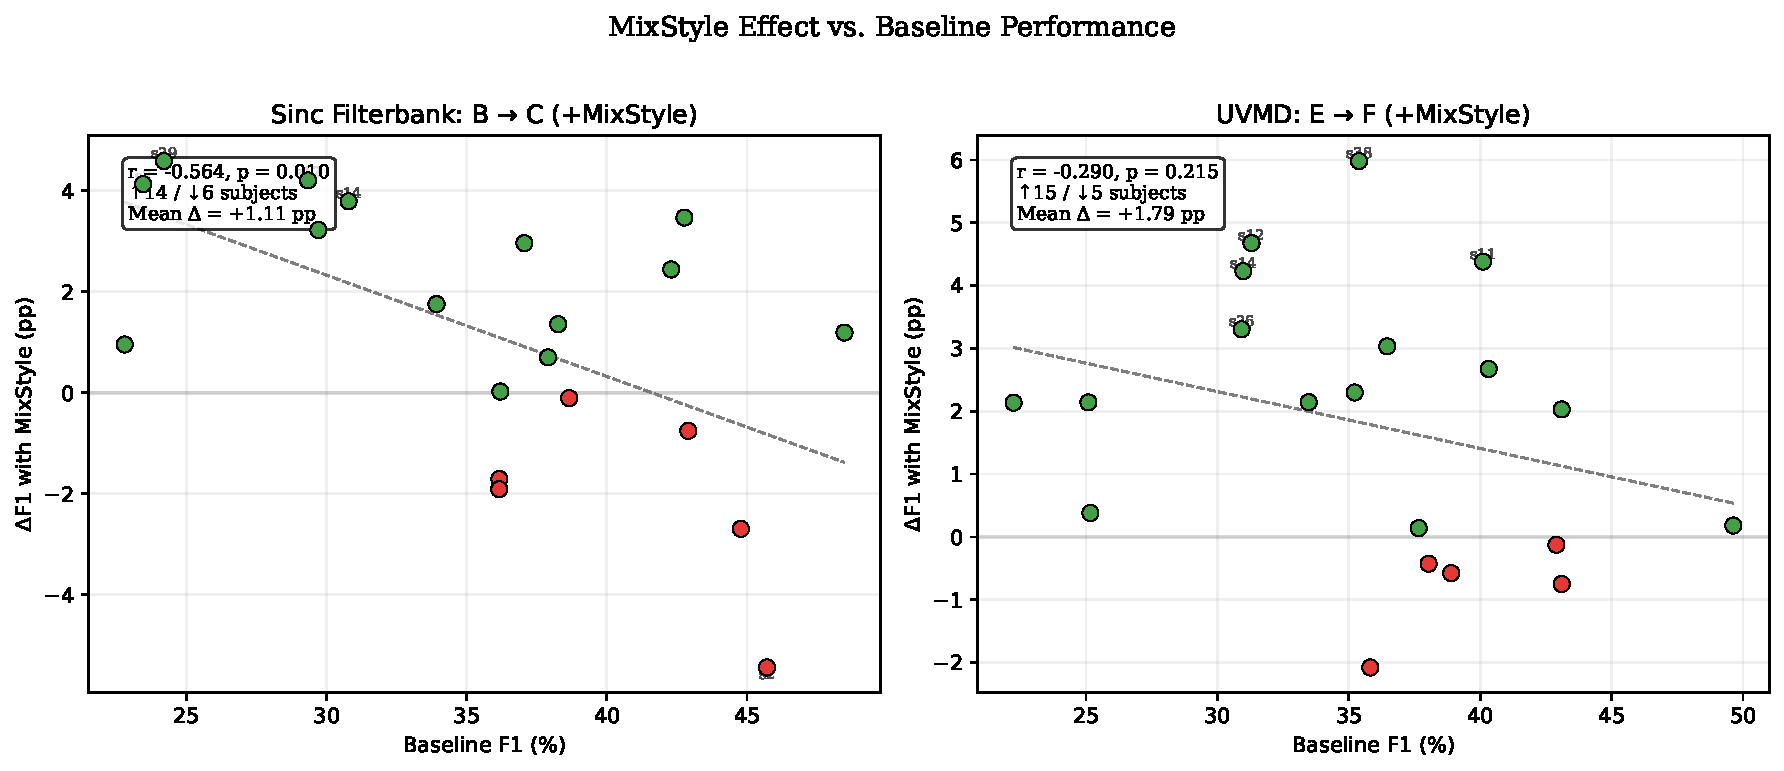
\includegraphics[width=\columnwidth]{fig_mixstyle_delta_correlation.pdf}
\caption{Per-subject \mixstyle{} F1 gain vs.\ baseline F1. Left: Sinc FB (B$\to$C), significant negative correlation. Right: \uvmd{} (E$\to$F), similar trend.}
\label{fig:mixstyle_corr}
\end{figure}

% ======================================================================
%  VII. ANALYSIS AND DISCUSSION
% ======================================================================
\section{Analysis and Discussion}
\label{sec:discussion}

\subsection{Decomposition as the Primary Confirmed Effect}
The H6 ablation shows decomposition (+3.68\pp{}, $d$\,=\,1.25, $p_{\mathrm{Holm}}$\,$<$\,0.003) contributes roughly three times more than \mixstyle{} (+1.11\pp{}, $d$\,=\,0.42, $p_{\mathrm{uncorr.}}$\,=\,0.07).
This ratio is consistent with the H1 observation that frequency structure is a major axis of subject-specific variation.
By isolating sub-bands, the per-band encoders can specialize: low-frequency encoders focus on motor-unit patterns (high Fisher ratio), while high-frequency encoders can learn to suppress noise (high normalized CV).
The \mixstyle{} effect on fixed Sinc decomposition (H3, H6~B$\to$C) remains exploratory: it does not pass Holm correction within Family~B.
On the learnable \uvmd{} frontend (H7), the effect is confirmatory ($p_{\mathrm{Holm}}$\,$<$\,0.01, $d$\,=\,0.84), suggesting that the benefit may depend on the frontend type or on the larger effect size achievable with adaptive decomposition.
We caution against interpreting \mixstyle{} as universally beneficial for sEMG; the evidence is mixed and frontend-dependent.

\subsection{H8: Learned Parameter Gradient as Descriptive Evidence}
The H8 experiment shows that a network optimized purely for classification loss learns $\alpha_k$ and $p_k$ that increase monotonically from low to high frequency bands, mirroring the H1~observation.
The Sinc frontend exhibits a 10$\times$ ratio ($\alpha_4/\alpha_1$\,=\,16.3/1.6), with Spearman $\rho$\,=\,0.775 ($p$\,$<$\,$10^{-16}$).

However, this evidence is \emph{descriptive}: the correlation between learned parameters and band index is an observation about the optimization outcome, not a controlled experiment.
The reversed-gradient ablation (UVMD: $-$0.97\pp{}, $p_{\mathrm{uncorr.}}$\,=\,0.064, 15/20~wins) provides a partial causal control, but the effect is small and non-significant.
We interpret the parameter gradient as \emph{suggestive} of a frequency-dependent structure, consistent with H1 but not independently confirming it through controlled manipulation.

The overall reduction in $p_k$ from initialization (0.5 to $<$0.001--0.04) is itself noteworthy: the network determines that the commonly used $p$\,=\,0.5 over-regularizes, and that low-frequency bands should receive essentially no style mixing.
If replicated on additional datasets, this finding could inform practical design choices for per-band augmentation.

\subsection{SCG-Net: Per-Band Style Removal}
The progression H1$\to$H8$\to$H9 traces a methodological arc: \emph{observe} the frequency-dependent variability (H1), examine whether learned augmentation parameters reflect it (H8, descriptive), then test whether encoding it as an architectural prior helps (H9).
The SCG gate differs from MixStyle: instead of training-time augmentation, it \emph{permanently removes} subject-specific variation from selected bands at both training and inference time.
The near-binary gate values ($\gamma_4$\,=\,0.998, $\gamma_{1\text{--}3}$\,$<$\,0.001) suggest that the optimal strategy is a hard frequency-dependent partition, though this conclusion is conditioned on our specific architecture and dataset.

The +6.86\pp{} advantage of SCG over uniform IN (\cref{tab:h9}) quantifies the cost of frequency-agnostic normalization.
However, SCG-Net (35.65\% F1) does not exceed the MixStyle-based pipeline (37.19--37.69\% F1), indicating that selective style \emph{removal} is less effective than style \emph{augmentation} for overall generalization.
SCG-Net's primary value in this study is as a diagnostic tool that confirms the binary content/style partition across frequency bands, rather than as a state-of-the-art architecture.

\subsection{Why Hard Normalization Fails}
Instance Normalization removes \emph{all} first- and second-order statistics, including channel-wise amplitude patterns that carry gesture information (which channels activate, and how strongly).
In contrast, \mixstyle{} only \emph{interpolates} between subjects' statistics, preserving the overall distribution structure while increasing training-time diversity.
The H8 experiment is consistent with this interpretation: learned parameters indicate minimal style mixing in low-frequency bands and selective mixing in high-frequency bands, though this is descriptive evidence (see~\cref{sec:h8}).
SCG-Net (H9) provides complementary evidence: when given a per-band gate ($\gamma_k \in [0,1]$), the network removes style only from the highest band ($\gamma_4 \approx 1$) and preserves it in all others.

\subsection{Why Adversarial Disentanglement Harms Performance}
Adversarial disentanglement (GRL) assumes that a representation can be split into subject-invariant ``content'' and subject-specific ``style'' components.
In our experiments, this assumption appears to fail: the amplitude pattern across 12 electrodes likely encodes both the gesture (which muscles activate) \emph{and} the subject's physiology (electrode placement, muscle mass, subcutaneous fat).
Forcing orthogonality between content and style projections may destroy gesture-relevant information.
The MI-minimization variant shows similar degradation.

We note that this conclusion is specific to the adversarial/MI-based disentanglement mechanisms tested in H4.
Separate exploratory experiments on a reduced 5-subject subset suggest that other disentanglement approaches (e.g., channel-contrastive with Group DRO) may avoid this failure mode, but these results cannot be compared directly with the 20-subject findings.

\subsection{Batch-Size Confound}
\label{sec:batchsize}

A limitation of this study is the change in batch size between experimental series: H2--H5 used batch\_size\,=\,64, while H6 used batch\_size\,=\,512.
This difference was introduced for computational efficiency in the unified ablation but has several implications:
\begin{itemize}
    \item \textbf{Absolute F1 values differ across series.} For example, the raw CNN baseline is 34.90\% in H2 (bs=64) vs.\ 32.40\% in H6 (bs=512). The Sinc+\mixstyle{} configuration is 37.95\% in H3 vs.\ 37.19\% in H6. These are \emph{not} directly comparable.
    \item \textbf{Batch size affects BatchNorm and \mixstyle{}.} Larger batches provide better BatchNorm statistics but reduce the diversity of \mixstyle{} pairings within a batch, potentially weakening the augmentation effect.
    \item \textbf{Component attributions from H6 are internally consistent} (same batch size throughout), but the absolute magnitudes may differ from what would be observed at batch\_size\,=\,64.
\end{itemize}
To verify that the H7 conclusion is robust to this confound, we replicated H7 Variant~F (\uvmd{}+\mixstyle{}) at batch\_size\,=\,64 (matching H2--H5).
The result---37.69\%\,$\pm$\,6.85---is not significantly different from the bs=512 run (37.58\%\,$\pm$\,6.39; paired Wilcoxon $p$\,=\,0.67), confirming that the \uvmd{}+\mixstyle{} effect is batch-size--invariant.
The bs=512 E$\to$F comparison remains internally consistent and is reported in \cref{tab:h7}.

\subsection{Limitations}
\begin{enumerate}
    \item \textbf{Single dataset and exercise.} All results are on NinaPro DB2 E1 (10~gestures, 12~channels, 2000\,Hz). Generalization to other NinaPro databases, exercises, electrode configurations, or recording hardware is untested.
    \item \textbf{Subset of subjects.} We use 20 of 40 available subjects. While chosen to span the full database range, this limits external validity.
    \item \textbf{Batch-size confound.} As discussed in \cref{sec:batchsize}, the change in batch size between H2--H5 and H6 complicates cross-table comparisons. The H7 main result has been replicated at batch\_size\,=\,64 ($p$\,=\,0.67 vs.\ original), but the H6 ablation was not re-run.
    \item \textbf{Mixed evidence for \mixstyle{}.} Per-band \mixstyle{} reaches confirmatory significance only on the learnable \uvmd{} frontend (H7). On fixed Sinc, the effect is consistent but exploratory. The benefit should not be treated as established until replicated.
    \item \textbf{H8 is descriptive.} The learned parameter gradient is an observational finding from parameter inspection, not a controlled comparison. The reversed-gradient ablation is small and non-significant. Conclusions about ``the network learning the H1 gradient'' should be interpreted cautiously.
    \item \textbf{SCG-Net comparison is narrow.} SCG-Net is compared against uniform IN (an intentionally weak baseline) and MixStyle variants, but not against other domain generalization architectures. Its value in this study is primarily diagnostic.
    \item \textbf{No real-time evaluation.} All experiments are offline; latency and computational constraints of embedded deployment are not addressed.
    \item \textbf{Novelty.} Frequency decomposition and \mixstyle{} are established methods; our contribution is their systematic per-band evaluation for cross-subject sEMG. The Spectral Content Gate is a novel but simple architectural element whose broader applicability remains untested.
\end{enumerate}

% ======================================================================
%  VIII. CONCLUSION
% ======================================================================
\section{Conclusion}
\label{sec:conclusion}

We presented a hypothesis-driven investigation (H1--H9) of frequency-aware processing for cross-subject sEMG gesture recognition on NinaPro DB2 (20~subjects, 10~gestures, LOSO).

\paragraph{Confirmatory findings ($p_{\mathrm{Holm}}$\,$<$\,0.05).}
\begin{itemize}
    \item $K$\,=\,4 frequency decomposition adds +3.7\pp{} F1 ($d$\,=\,1.25) over a raw-signal baseline (H6; also confirmed in H2).
    \item Per-band \mixstyle{} on learnable \uvmd{} decomposition adds +1.8\pp{} ($d$\,=\,0.84, H7). On fixed Sinc decomposition, the effect is consistent in direction but remains exploratory.
    \item Hard Instance Normalization is strongly harmful ($-$7 to $-$8.5\pp{}).
    \item Adversarial and MI-based disentanglement degrade performance ($-$2.6 to $-$4.3\pp{}) under the architectures tested.
    \item SCG-Net's per-band gate outperforms uniform Instance Normalization by +6.86\pp{} ($p_{\mathrm{Holm}}$\,$<$\,0.001).
\end{itemize}

\paragraph{Descriptive and exploratory findings.}
\begin{itemize}
    \item Per-band \mixstyle{} on fixed Sinc: +1.1--1.7\pp{}, consistent direction but not confirmed after correction.
    \item Adaptive Per-Band \mixstyle{} (H8) learns parameters correlated with the H1~gradient ($\alpha_4/\alpha_1$\,=\,10$\times$, $\rho$\,=\,0.78), but this is descriptive evidence from parameter inspection, not a controlled comparison.
    \item SCG-Net learns a near-binary gate partition ($\gamma_4$\,=\,0.998, $\gamma_{1\text{--}3}$\,$<$\,0.001), consistent with H1 but based on the same architectural framework.
\end{itemize}

The combined pipeline achieves 37.7\% macro-F1 (\uvmd{}+\mixstyle{}, replicated at two batch sizes), compared with the published baseline of 33.5\%.
These results are obtained on a single dataset with a subset of subjects and should be validated on other sEMG benchmarks and electrode configurations before broader conclusions are drawn.
Within these limitations, our findings suggest that frequency-dependent inter-subject variability is a significant structural property of sEMG that can be addressed through per-band processing, with decomposition providing the largest confirmed benefit.

% ======================================================================
%  REFERENCES
% ======================================================================
\bibliographystyle{IEEEtran}
% TODO: Create references.bib with all cited works
\begin{thebibliography}{99}

\bibitem{atzori2016deep}
M.~Atzori \etal, ``Deep learning with convolutional neural networks applied to electromyography data: A resource for the classification of movements for prosthetic hands,'' \textit{Front. Neurorobot.}, vol.~10, 2016.

\bibitem{atzori2014electromyography}
M.~Atzori \etal, ``Electromyography data for non-invasive naturally-controlled robotic hand prostheses,'' \textit{Sci. Data}, vol.~1, p.~140053, 2014.

\bibitem{farina2014extraction}
D.~Farina \etal, ``The extraction of neural information from the surface EMG for the control of upper-limb prostheses: emerging avenues and challenges,'' \textit{IEEE Trans. Neural Syst. Rehabil. Eng.}, vol.~22, no.~4, pp.~797--809, 2014.

\bibitem{saponas2009enabling}
T.~S.~Saponas \etal, ``Enabling always-available input with muscle-computer interfaces,'' in \textit{Proc. UIST}, 2009.

\bibitem{campbell2020current}
E.~Campbell \etal, ``Current trends and confounding factors in myoelectric control: Limb position and contraction intensity,'' \textit{Sensors}, vol.~20, no.~6, 2020.

\bibitem{cote2019deep}
U.~C\^{o}t\'{e}-Allard \etal, ``Deep learning for electromyographic hand gesture signal classification using transfer learning,'' \textit{IEEE Trans. Neural Syst. Rehabil. Eng.}, vol.~27, no.~4, pp.~760--771, 2019.

\bibitem{du2017surface}
Y.~Du \etal, ``Surface EMG-based inter-session gesture recognition enhanced by deep domain adaptation,'' \textit{Sensors}, vol.~17, no.~3, 2017.

\bibitem{phinyomark2012feature}
A.~Phinyomark \etal, ``Feature reduction and selection for EMG signal classification,'' \textit{Expert Syst. Appl.}, vol.~39, no.~8, pp.~7420--7431, 2012.

\bibitem{golovan2025benchmark}
K.~Golovan and I.~Zvereva, ``A reproducible benchmark for zero-shot cross-subject hand gesture recognition using sEMG signals,'' 2025.

\bibitem{dragomiretskiy2014variational}
K.~Dragomiretskiy and D.~Zosso, ``Variational mode decomposition,'' \textit{IEEE Trans. Signal Process.}, vol.~62, no.~3, pp.~531--544, 2014.

\bibitem{ravanelli2018speaker}
M.~Ravanelli and Y.~Bengio, ``Speaker recognition from raw waveform with SincNet,'' in \textit{Proc. SLT}, 2018.

\bibitem{zhou2021mixstyle}
K.~Zhou \etal, ``Domain generalization with MixStyle,'' in \textit{Proc. ICLR}, 2021.

\bibitem{hudgins1993new}
B.~Hudgins, P.~Parker, and R.~N.~Scott, ``A new strategy for multifunction myoelectric control,'' \textit{IEEE Trans. Biomed. Eng.}, vol.~40, no.~1, pp.~82--94, 1993.

\bibitem{englehart2003robust}
K.~Englehart and B.~Hudgins, ``A robust, real-time control scheme for multifunction myoelectric control,'' \textit{IEEE Trans. Biomed. Eng.}, vol.~50, no.~7, pp.~848--854, 2003.

\bibitem{scheme2011electromyogram}
E.~Scheme and K.~Englehart, ``Electromyogram pattern recognition for control of powered upper-limb prostheses: State of the art and challenges for clinical use,'' \textit{J. Rehabil. Res. Dev.}, vol.~48, no.~6, pp.~643--659, 2011.

\bibitem{pizzolato2017comparison}
S.~Pizzolato \etal, ``Comparison of six electromyography acquisition setups on hand movement classification tasks,'' \textit{PLoS ONE}, vol.~12, no.~10, e0186132, 2017.

\bibitem{zhai2017self}
X.~Zhai \etal, ``Self-recalibrating surface EMG pattern recognition for neuroprosthesis control based on convolutional neural network,'' \textit{Front. Neurosci.}, vol.~11, 379, 2017.

\bibitem{wei2019multistream}
W.~Wei \etal, ``A multi-stream convolutional neural network for sEMG-based gesture recognition in muscle-computer interface,'' \textit{Pattern Recognit. Lett.}, vol.~119, pp.~131--138, 2019.

\bibitem{ketyko2019domain}
I.~Ketyk\'{o}, F.~Kov\'{a}cs, and K.~Z.~Varga, ``Domain adaptation for sEMG-based gesture recognition with recurrent neural networks,'' in \textit{Proc. IJCNN}, 2019.

\bibitem{huang1998empirical}
N.~E.~Huang \etal, ``The empirical mode decomposition and the Hilbert spectrum for nonlinear and non-stationary time series analysis,'' \textit{Proc. R. Soc. Lond. A}, vol.~454, pp.~903--995, 1998.

\bibitem{rehman2010multivariate}
N.~Rehman and D.~P.~Mandic, ``Multivariate empirical mode decomposition,'' \textit{Proc. R. Soc. A}, vol.~466, pp.~1291--1302, 2010.

\bibitem{englehart1999wavelet}
K.~Englehart \etal, ``Classification of the myoelectric signal using time-frequency based representations,'' \textit{Med. Biol. Eng. Comput.}, vol.~37, no.~4, pp.~526--532, 1999.

\bibitem{phinyomark2018emg_frequency}
A.~Phinyomark and E.~Scheme, ``EMG pattern recognition in the era of big data and deep learning,'' \textit{Big Data Cogn. Comput.}, vol.~2, no.~3, 21, 2018.

\bibitem{borra2020sincnet_eeg}
D.~Borra \etal, ``Interpretable and lightweight convolutional neural network for EEG decoding: Application to movement execution and imagination,'' \textit{Neural Netw.}, vol.~129, pp.~55--74, 2020.

\bibitem{ioffe2015batch}
S.~Ioffe and C.~Szegedy, ``Batch normalization: Accelerating deep network training by reducing internal covariate shift,'' in \textit{Proc. ICML}, 2015.

\bibitem{ulyanov2016instance}
D.~Ulyanov, A.~Vedaldi, and V.~Lempitsky, ``Instance normalization: The missing ingredient for fast stylization,'' \textit{arXiv:1607.08022}, 2016.

\bibitem{huang2017adain}
X.~Huang and S.~Belongie, ``Arbitrary style transfer in real-time with adaptive instance normalization,'' in \textit{Proc. ICCV}, 2017.

\bibitem{sagawa2020distributionally}
S.~Sagawa \etal, ``Distributionally robust neural networks for group shifts: On the importance of regularization for worst-case generalization,'' in \textit{Proc. ICLR}, 2020.

\bibitem{arjovsky2019invariant}
M.~Arjovsky \etal, ``Invariant risk minimization,'' \textit{arXiv:1907.02893}, 2019.

\bibitem{ganin2016domain}
Y.~Ganin \etal, ``Domain-adversarial training of neural networks,'' \textit{J. Mach. Learn. Res.}, vol.~17, no.~59, pp.~1--35, 2016.

\bibitem{wang2022generalizing}
J.~Wang \etal, ``Generalizing to unseen domains: A survey on domain generalization,'' \textit{IEEE Trans. Knowl. Data Eng.}, vol.~35, no.~8, pp.~8052--8072, 2023.

\bibitem{holm1979simple}
S.~Holm, ``A simple sequentially rejective multiple test procedure,'' \textit{Scandinavian J. Statistics}, vol.~6, no.~2, pp.~65--70, 1979.

\end{thebibliography}

\end{document}
